\documentclass[twoside]{book}

% Packages required by doxygen
\usepackage{fixltx2e}
\usepackage{calc}
\usepackage{doxygen}
\usepackage[export]{adjustbox} % also loads graphicx
\usepackage{graphicx}
\usepackage[utf8]{inputenc}
\usepackage{makeidx}
\usepackage{multicol}
\usepackage{multirow}
\PassOptionsToPackage{warn}{textcomp}
\usepackage{textcomp}
\usepackage[nointegrals]{wasysym}
\usepackage[table]{xcolor}

% Font selection
\usepackage[T1]{fontenc}
\usepackage[scaled=.90]{helvet}
\usepackage{courier}
\usepackage{amssymb}
\usepackage{sectsty}
\renewcommand{\familydefault}{\sfdefault}
\allsectionsfont{%
  \fontseries{bc}\selectfont%
  \color{darkgray}%
}
\renewcommand{\DoxyLabelFont}{%
  \fontseries{bc}\selectfont%
  \color{darkgray}%
}
\newcommand{\+}{\discretionary{\mbox{\scriptsize$\hookleftarrow$}}{}{}}

% Page & text layout
\usepackage{geometry}
\geometry{%
  a4paper,%
  top=2.5cm,%
  bottom=2.5cm,%
  left=2.5cm,%
  right=2.5cm%
}
\tolerance=750
\hfuzz=15pt
\hbadness=750
\setlength{\emergencystretch}{15pt}
\setlength{\parindent}{0cm}
\setlength{\parskip}{3ex plus 2ex minus 2ex}
\makeatletter
\renewcommand{\paragraph}{%
  \@startsection{paragraph}{4}{0ex}{-1.0ex}{1.0ex}{%
    \normalfont\normalsize\bfseries\SS@parafont%
  }%
}
\renewcommand{\subparagraph}{%
  \@startsection{subparagraph}{5}{0ex}{-1.0ex}{1.0ex}{%
    \normalfont\normalsize\bfseries\SS@subparafont%
  }%
}
\makeatother

% Headers & footers
\usepackage{fancyhdr}
\pagestyle{fancyplain}
\fancyhead[LE]{\fancyplain{}{\bfseries\thepage}}
\fancyhead[CE]{\fancyplain{}{}}
\fancyhead[RE]{\fancyplain{}{\bfseries\leftmark}}
\fancyhead[LO]{\fancyplain{}{\bfseries\rightmark}}
\fancyhead[CO]{\fancyplain{}{}}
\fancyhead[RO]{\fancyplain{}{\bfseries\thepage}}
\fancyfoot[LE]{\fancyplain{}{}}
\fancyfoot[CE]{\fancyplain{}{}}
\fancyfoot[RE]{\fancyplain{}{\bfseries\scriptsize Generated by Doxygen }}
\fancyfoot[LO]{\fancyplain{}{\bfseries\scriptsize Generated by Doxygen }}
\fancyfoot[CO]{\fancyplain{}{}}
\fancyfoot[RO]{\fancyplain{}{}}
\renewcommand{\footrulewidth}{0.4pt}
\renewcommand{\chaptermark}[1]{%
  \markboth{#1}{}%
}
\renewcommand{\sectionmark}[1]{%
  \markright{\thesection\ #1}%
}

% Indices & bibliography
\usepackage{natbib}
\usepackage[titles]{tocloft}
\setcounter{tocdepth}{3}
\setcounter{secnumdepth}{5}
\makeindex

% Hyperlinks (required, but should be loaded last)
\usepackage{ifpdf}
\ifpdf
  \usepackage[pdftex,pagebackref=true]{hyperref}
\else
  \usepackage[ps2pdf,pagebackref=true]{hyperref}
\fi
\hypersetup{%
  colorlinks=true,%
  linkcolor=blue,%
  citecolor=blue,%
  unicode%
}

% Custom commands
\newcommand{\clearemptydoublepage}{%
  \newpage{\pagestyle{empty}\cleardoublepage}%
}

\usepackage{caption}
\captionsetup{labelsep=space,justification=centering,font={bf},singlelinecheck=off,skip=4pt,position=top}

%===== C O N T E N T S =====

\begin{document}

% Titlepage & ToC
\hypersetup{pageanchor=false,
             bookmarksnumbered=true,
             pdfencoding=unicode
            }
\pagenumbering{roman}
\begin{titlepage}
\vspace*{7cm}
\begin{center}%
{\Large Autonomous Racing \\[1ex]\large 1 }\\
\vspace*{1cm}
{\large Generated by Doxygen 1.8.11}\\
\end{center}
\end{titlepage}
\clearemptydoublepage
\tableofcontents
\clearemptydoublepage
\pagenumbering{arabic}
\hypersetup{pageanchor=true}

%--- Begin generated contents ---
\chapter{Autonomous Racing Project Group}
\label{index}\hypertarget{index}{}\section*{Introduction}

This is the introduction.\hypertarget{index_install_sec}{}\section{Installation}\label{index_install_sec}
\hypertarget{index_step1}{}\subsection{Step 1\+: Opening the box}\label{index_step1}
etc... 
\chapter{Project Title}
\label{md__home_travis_build_Autonomous-Racing-PG_ros.package_docs_master_README}
\hypertarget{md__home_travis_build_Autonomous-Racing-PG_ros.package_docs_master_README}{}
Autonomous Racing -\/ Project Group -\/ TU Dortmund

\href{https://travis-ci.com/Autonomous-Racing-PG/ros.package}{\tt }

\subsection*{Getting Started}

These instructions will get you a copy of the project up and running

\#\#\# Install missing system dependencies 
\begin{DoxyCode}
1 sudo apt install libsdl2-dev python-pip clang-format
2 pip install torch autopep8
3 
4 # RangeLibc
5 sudo pip uninstall pip && sudo apt install python-pip
6 pip install cython
7 git clone http://github.com/kctess5/range\_libc
8 cd range\_libc/pywrapper
9 # Either:
10 ./compile.sh            # on VM
11 # Or:
12 ./compile\_with\_cuda.sh  # on car - compiles GPU ray casting methods
\end{DoxyCode}


\subsubsection*{Clone the Project}


\begin{DoxyCode}
1 git clone --recurse-submodules https://github.com/Autonomous-Racing-PG/ros.package.git arpg
2 cd arpg
\end{DoxyCode}


\subsubsection*{Move to R\+OS Workspace}


\begin{DoxyCode}
1 cd ros\_ws
\end{DoxyCode}


\#\#\# Install missing R\+OS dependencies 
\begin{DoxyCode}
1 rosdep install -y --from-paths src --ignore-src --rosdistro $\{ROS\_DISTRO\}
\end{DoxyCode}


\subsubsection*{Build R\+OS packages}


\begin{DoxyCode}
1 catkin\_make
\end{DoxyCode}


\subsubsection*{Run routines}


\begin{DoxyCode}
1 source devel/setup.bash (or setup.zsh)
\end{DoxyCode}


Now several routines can be started by executing the launch-\/files inside the {\bfseries launch/} directory. E.\+g.


\begin{DoxyCode}
1 roslaunch launch/gazebo\_car-teleop.launch
\end{DoxyCode}


\subsubsection*{Run tests}


\begin{DoxyCode}
1 catkin\_make run\_tests
\end{DoxyCode}


\subsection*{Building a map with Cartographer}

There are two bash scripts in the {\ttfamily scripts} folder which use \href{https://github.com/googlecartographer/cartographer_ros}{\tt Cartographer} to create a map of a racetrack. This map can then be used for different purposes, for example in the R\+OS navigation stack.


\begin{DoxyItemize}
\item To build a map while a roscore is running and providing sensor data, use the {\ttfamily cartographer\+\_\+online} script.
\item To build a map from a rosbag, use the {\ttfamily cartographer\+\_\+offline} script. The rosbag must provide range data on the rostopic {\ttfamily /scan} and a transformation tree on {\ttfamily /tf}; depending on your configuration of cartographer in {\ttfamily car\+\_\+cartographer/config} it may need to also have odometry data on {\ttfamily /odom} or I\+MU data on {\ttfamily /imu}.
\end{DoxyItemize}


\begin{DoxyCode}
1 # Either:
2 ./scripts/cartographer\_online.sh
3 # Or:
4 ./scripts/cartographer\_offline.sh /absolute/path/to/rosbag
\end{DoxyCode}


\subsection*{Documentation}


\begin{DoxyItemize}
\item For general information and documentation checkout the \href{https://github.com/Autonomous-Racing-PG/ros.package/wiki}{\tt wiki page}.
\item For source code documentation checkout the auto-\/generated \href{https://autonomous-racing-pg.github.io/ros.package/html/index.html}{\tt Doxygen documentation}.
\end{DoxyItemize}

\subsection*{License}

This project (exluded git submodules) is licensed under the M\+IT and G\+P\+Lv3 dual licensed -\/ see the \href{MIT.LICENSE}{\tt M\+I\+T.\+L\+I\+C\+E\+N\+SE} and \href{GPLv3.LICENSE}{\tt G\+P\+Lv3.\+L\+I\+C\+E\+N\+SE} file for details

\subsection*{Acknowledgments}


\begin{DoxyItemize}
\item TU Dortmund 
\end{DoxyItemize}
\chapter{Namespace Index}
\section{Namespace List}
Here is a list of all namespaces with brief descriptions\+:\begin{DoxyCompactList}
\item\contentsline{section}{\hyperlink{namespacecar__config}{car\+\_\+config} }{\pageref{namespacecar__config}}{}
\item\contentsline{section}{\hyperlink{namespacecircle}{circle} }{\pageref{namespacecircle}}{}
\item\contentsline{section}{\hyperlink{namespacelap__timer}{lap\+\_\+timer} }{\pageref{namespacelap__timer}}{}
\item\contentsline{section}{\hyperlink{namespacerviz__geometry}{rviz\+\_\+geometry} }{\pageref{namespacerviz__geometry}}{}
\item\contentsline{section}{\hyperlink{namespacesimulation}{simulation} }{\pageref{namespacesimulation}}{}
\item\contentsline{section}{\hyperlink{namespacespeedometer}{speedometer} }{\pageref{namespacespeedometer}}{}
\item\contentsline{section}{\hyperlink{namespacewallfollowing}{wallfollowing} }{\pageref{namespacewallfollowing}}{}
\end{DoxyCompactList}

\chapter{Class Index}
\section{Class List}
Here are the classes, structs, unions and interfaces with brief descriptions\+:\begin{DoxyCompactList}
\item\contentsline{section}{\hyperlink{class_autonomous_control}{Autonomous\+Control} }{\pageref{class_autonomous_control}}{}
\item\contentsline{section}{\hyperlink{class_car_controller}{Car\+Controller} }{\pageref{class_car_controller}}{}
\item\contentsline{section}{\hyperlink{class_d_m_s_controller}{D\+M\+S\+Controller} }{\pageref{class_d_m_s_controller}}{}
\item\contentsline{section}{\hyperlink{class_drive_parameters_multiplexer}{Drive\+Parameters\+Multiplexer} }{\pageref{class_drive_parameters_multiplexer}}{}
\item\contentsline{section}{\hyperlink{class_drive_parameters_source}{Drive\+Parameters\+Source} }{\pageref{class_drive_parameters_source}}{}
\item\contentsline{section}{\hyperlink{class_emergency_stop}{Emergency\+Stop} }{\pageref{class_emergency_stop}}{}
\item\contentsline{section}{\hyperlink{class_joystick_controller}{Joystick\+Controller} }{\pageref{class_joystick_controller}}{}
\item\contentsline{section}{\hyperlink{class_keyboard_controller}{Keyboard\+Controller} }{\pageref{class_keyboard_controller}}{}
\item\contentsline{section}{\hyperlink{class_navigation_stack_control_converter}{Navigation\+Stack\+Control\+Converter} \\*This converter class converts \char`\"{}cmd\+\_\+vel\char`\"{} messages to \char`\"{}drive\+\_\+param\char`\"{} messages. The linear and angular velocity has to be transformed to linear velocity and steering angle. T\+O\+DO\+: Differential drive? }{\pageref{class_navigation_stack_control_converter}}{}
\item\contentsline{section}{\hyperlink{class_v_e_s_c_simulation_driver}{V\+E\+S\+C\+Simulation\+Driver} \\*Class to convert Drive Parameter Messages into single messages }{\pageref{class_v_e_s_c_simulation_driver}}{}
\item\contentsline{section}{\hyperlink{class_v_e_s_c_simulator}{V\+E\+S\+C\+Simulator} }{\pageref{class_v_e_s_c_simulator}}{}
\item\contentsline{section}{\hyperlink{class_wall_following}{Wall\+Following} }{\pageref{class_wall_following}}{}
\end{DoxyCompactList}

\chapter{File Index}
\section{File List}
Here is a list of all files with brief descriptions\+:\begin{DoxyCompactList}
\item\contentsline{section}{/home/travis/build/\+Autonomous-\/\+Racing-\/\+P\+G/ros.\+package/docs/master/ros\+\_\+ws/src/autonomous/src/\hyperlink{autonomous__control_8cpp}{autonomous\+\_\+control.\+cpp} }{\pageref{autonomous__control_8cpp}}{}
\item\contentsline{section}{/home/travis/build/\+Autonomous-\/\+Racing-\/\+P\+G/ros.\+package/docs/master/ros\+\_\+ws/src/autonomous/src/\hyperlink{wall__following_8cpp}{wall\+\_\+following.\+cpp} }{\pageref{wall__following_8cpp}}{}
\item\contentsline{section}{/home/travis/build/\+Autonomous-\/\+Racing-\/\+P\+G/ros.\+package/docs/master/ros\+\_\+ws/src/car\+\_\+control/include/\hyperlink{car__controller_8h}{car\+\_\+controller.\+h} }{\pageref{car__controller_8h}}{}
\item\contentsline{section}{/home/travis/build/\+Autonomous-\/\+Racing-\/\+P\+G/ros.\+package/docs/master/ros\+\_\+ws/src/car\+\_\+control/src/\hyperlink{car__controller_8cpp}{car\+\_\+controller.\+cpp} }{\pageref{car__controller_8cpp}}{}
\item\contentsline{section}{/home/travis/build/\+Autonomous-\/\+Racing-\/\+P\+G/ros.\+package/docs/master/ros\+\_\+ws/src/car\+\_\+control/test/\hyperlink{test__car__control_8cpp}{test\+\_\+car\+\_\+control.\+cpp} }{\pageref{test__car__control_8cpp}}{}
\item\contentsline{section}{/home/travis/build/\+Autonomous-\/\+Racing-\/\+P\+G/ros.\+package/docs/master/ros\+\_\+ws/src/simulation/racer\+\_\+control/include/\hyperlink{drive__param__converter_8h}{drive\+\_\+param\+\_\+converter.\+h} }{\pageref{drive__param__converter_8h}}{}
\item\contentsline{section}{/home/travis/build/\+Autonomous-\/\+Racing-\/\+P\+G/ros.\+package/docs/master/ros\+\_\+ws/src/simulation/racer\+\_\+control/src/\hyperlink{drive__param__converter_8cpp}{drive\+\_\+param\+\_\+converter.\+cpp} }{\pageref{drive__param__converter_8cpp}}{}
\item\contentsline{section}{/home/travis/build/\+Autonomous-\/\+Racing-\/\+P\+G/ros.\+package/docs/master/ros\+\_\+ws/src/simulation/racer\+\_\+control/src/\hyperlink{racer__control_2src_2main_8cpp}{main.\+cpp} }{\pageref{racer__control_2src_2main_8cpp}}{}
\item\contentsline{section}{/home/travis/build/\+Autonomous-\/\+Racing-\/\+P\+G/ros.\+package/docs/master/ros\+\_\+ws/src/simulation/racer\+\_\+sensors/include/\hyperlink{racer__odometry_8h}{racer\+\_\+odometry.\+h} }{\pageref{racer__odometry_8h}}{}
\item\contentsline{section}{/home/travis/build/\+Autonomous-\/\+Racing-\/\+P\+G/ros.\+package/docs/master/ros\+\_\+ws/src/simulation/racer\+\_\+sensors/src/\hyperlink{main__racer__odometry_8cpp}{main\+\_\+racer\+\_\+odometry.\+cpp} }{\pageref{main__racer__odometry_8cpp}}{}
\item\contentsline{section}{/home/travis/build/\+Autonomous-\/\+Racing-\/\+P\+G/ros.\+package/docs/master/ros\+\_\+ws/src/simulation/racer\+\_\+sensors/src/\hyperlink{racer__odometry_8cpp}{racer\+\_\+odometry.\+cpp} }{\pageref{racer__odometry_8cpp}}{}
\item\contentsline{section}{/home/travis/build/\+Autonomous-\/\+Racing-\/\+P\+G/ros.\+package/docs/master/ros\+\_\+ws/src/simulation/vesc\+\_\+sim/include/\hyperlink{car__config_8h}{car\+\_\+config.\+h} }{\pageref{car__config_8h}}{}
\item\contentsline{section}{/home/travis/build/\+Autonomous-\/\+Racing-\/\+P\+G/ros.\+package/docs/master/ros\+\_\+ws/src/simulation/vesc\+\_\+sim/include/\hyperlink{vesc__sim_8h}{vesc\+\_\+sim.\+h} }{\pageref{vesc__sim_8h}}{}
\item\contentsline{section}{/home/travis/build/\+Autonomous-\/\+Racing-\/\+P\+G/ros.\+package/docs/master/ros\+\_\+ws/src/simulation/vesc\+\_\+sim/include/\hyperlink{vesc__sim__driver_8h}{vesc\+\_\+sim\+\_\+driver.\+h} }{\pageref{vesc__sim__driver_8h}}{}
\item\contentsline{section}{/home/travis/build/\+Autonomous-\/\+Racing-\/\+P\+G/ros.\+package/docs/master/ros\+\_\+ws/src/simulation/vesc\+\_\+sim/src/\hyperlink{vesc__sim_2src_2main_8cpp}{main.\+cpp} }{\pageref{vesc__sim_2src_2main_8cpp}}{}
\item\contentsline{section}{/home/travis/build/\+Autonomous-\/\+Racing-\/\+P\+G/ros.\+package/docs/master/ros\+\_\+ws/src/simulation/vesc\+\_\+sim/src/\hyperlink{vesc__sim_8cpp}{vesc\+\_\+sim.\+cpp} }{\pageref{vesc__sim_8cpp}}{}
\item\contentsline{section}{/home/travis/build/\+Autonomous-\/\+Racing-\/\+P\+G/ros.\+package/docs/master/ros\+\_\+ws/src/simulation/vesc\+\_\+sim/src/\hyperlink{vesc__sim__driver_8cpp}{vesc\+\_\+sim\+\_\+driver.\+cpp} }{\pageref{vesc__sim__driver_8cpp}}{}
\item\contentsline{section}{/home/travis/build/\+Autonomous-\/\+Racing-\/\+P\+G/ros.\+package/docs/master/ros\+\_\+ws/src/teleoperation/include/\hyperlink{joystick__controller_8h}{joystick\+\_\+controller.\+h} }{\pageref{joystick__controller_8h}}{}
\item\contentsline{section}{/home/travis/build/\+Autonomous-\/\+Racing-\/\+P\+G/ros.\+package/docs/master/ros\+\_\+ws/src/teleoperation/include/\hyperlink{keyboard__controller_8h}{keyboard\+\_\+controller.\+h} }{\pageref{keyboard__controller_8h}}{}
\item\contentsline{section}{/home/travis/build/\+Autonomous-\/\+Racing-\/\+P\+G/ros.\+package/docs/master/ros\+\_\+ws/src/teleoperation/src/\hyperlink{joystick__controller_8cpp}{joystick\+\_\+controller.\+cpp} }{\pageref{joystick__controller_8cpp}}{}
\item\contentsline{section}{/home/travis/build/\+Autonomous-\/\+Racing-\/\+P\+G/ros.\+package/docs/master/ros\+\_\+ws/src/teleoperation/src/\hyperlink{keyboard__controller_8cpp}{keyboard\+\_\+controller.\+cpp} }{\pageref{keyboard__controller_8cpp}}{}
\end{DoxyCompactList}

\chapter{Namespace Documentation}
\hypertarget{namespacedrive__param__converter}{}\section{drive\+\_\+param\+\_\+converter Namespace Reference}
\label{namespacedrive__param__converter}\index{drive\+\_\+param\+\_\+converter@{drive\+\_\+param\+\_\+converter}}
\subsection*{Functions}
\begin{DoxyCompactItemize}
\item 
def \hyperlink{namespacedrive__param__converter_afdd5fa91c648e8545fae1cd833995f40}{set\+\_\+throttle\+\_\+steer} (data)
\item 
def \hyperlink{namespacedrive__param__converter_a14d9041f6f5fd041bfbea4f26cbe0155}{drive\+\_\+param\+\_\+converter} ()
\end{DoxyCompactItemize}
\subsection*{Variables}
\begin{DoxyCompactItemize}
\item 
int \hyperlink{namespacedrive__param__converter_aab4bf01f556d80bbeeb22edf8bf07611}{flag\+\_\+move} = 0
\end{DoxyCompactItemize}


\subsection{Function Documentation}
\index{drive\+\_\+param\+\_\+converter@{drive\+\_\+param\+\_\+converter}!drive\+\_\+param\+\_\+converter@{drive\+\_\+param\+\_\+converter}}
\index{drive\+\_\+param\+\_\+converter@{drive\+\_\+param\+\_\+converter}!drive\+\_\+param\+\_\+converter@{drive\+\_\+param\+\_\+converter}}
\subsubsection[{\texorpdfstring{drive\+\_\+param\+\_\+converter()}{drive_param_converter()}}]{\setlength{\rightskip}{0pt plus 5cm}def drive\+\_\+param\+\_\+converter.\+drive\+\_\+param\+\_\+converter (
\begin{DoxyParamCaption}
{}
\end{DoxyParamCaption}
)}\hypertarget{namespacedrive__param__converter_a14d9041f6f5fd041bfbea4f26cbe0155}{}\label{namespacedrive__param__converter_a14d9041f6f5fd041bfbea4f26cbe0155}


Definition at line 40 of file drive\+\_\+param\+\_\+converter.\+py.

\index{drive\+\_\+param\+\_\+converter@{drive\+\_\+param\+\_\+converter}!set\+\_\+throttle\+\_\+steer@{set\+\_\+throttle\+\_\+steer}}
\index{set\+\_\+throttle\+\_\+steer@{set\+\_\+throttle\+\_\+steer}!drive\+\_\+param\+\_\+converter@{drive\+\_\+param\+\_\+converter}}
\subsubsection[{\texorpdfstring{set\+\_\+throttle\+\_\+steer(data)}{set_throttle_steer(data)}}]{\setlength{\rightskip}{0pt plus 5cm}def drive\+\_\+param\+\_\+converter.\+set\+\_\+throttle\+\_\+steer (
\begin{DoxyParamCaption}
\item[{}]{data}
\end{DoxyParamCaption}
)}\hypertarget{namespacedrive__param__converter_afdd5fa91c648e8545fae1cd833995f40}{}\label{namespacedrive__param__converter_afdd5fa91c648e8545fae1cd833995f40}
\begin{DoxyVerb}This method get's called when new drive_parameters are published.
It then converts the single message into 6 new messages.
The first 4 are the velocity of each individual wheels (velocity of the car).
The last 2 are the steering hinge angle for each of the front wheels (steering angle of the car).

Args:
    data:   A drive_param message
\end{DoxyVerb}
 

Definition at line 9 of file drive\+\_\+param\+\_\+converter.\+py.



\subsection{Variable Documentation}
\index{drive\+\_\+param\+\_\+converter@{drive\+\_\+param\+\_\+converter}!flag\+\_\+move@{flag\+\_\+move}}
\index{flag\+\_\+move@{flag\+\_\+move}!drive\+\_\+param\+\_\+converter@{drive\+\_\+param\+\_\+converter}}
\subsubsection[{\texorpdfstring{flag\+\_\+move}{flag_move}}]{\setlength{\rightskip}{0pt plus 5cm}int drive\+\_\+param\+\_\+converter.\+flag\+\_\+move = 0}\hypertarget{namespacedrive__param__converter_aab4bf01f556d80bbeeb22edf8bf07611}{}\label{namespacedrive__param__converter_aab4bf01f556d80bbeeb22edf8bf07611}


Definition at line 7 of file drive\+\_\+param\+\_\+converter.\+py.


\chapter{Class Documentation}
\hypertarget{class_car_control}{}\section{Car\+Control Class Reference}
\label{class_car_control}\index{Car\+Control@{Car\+Control}}
\subsection*{Public Member Functions}
\begin{DoxyCompactItemize}
\item 
\hyperlink{class_car_control_a233b5d77ce5d0594a1d9e438cc8eb04e}{Car\+Control} ()
\end{DoxyCompactItemize}


\subsection{Detailed Description}


Definition at line 24 of file car\+\_\+control.\+cpp.



\subsection{Constructor \& Destructor Documentation}
\index{Car\+Control@{Car\+Control}!Car\+Control@{Car\+Control}}
\index{Car\+Control@{Car\+Control}!Car\+Control@{Car\+Control}}
\subsubsection[{\texorpdfstring{Car\+Control()}{CarControl()}}]{\setlength{\rightskip}{0pt plus 5cm}Car\+Control\+::\+Car\+Control (
\begin{DoxyParamCaption}
{}
\end{DoxyParamCaption}
)}\hypertarget{class_car_control_a233b5d77ce5d0594a1d9e438cc8eb04e}{}\label{class_car_control_a233b5d77ce5d0594a1d9e438cc8eb04e}


Definition at line 54 of file car\+\_\+control.\+cpp.



The documentation for this class was generated from the following file\+:\begin{DoxyCompactItemize}
\item 
/home/travis/build/\+Autonomous-\/\+Racing-\/\+P\+G/ros.\+package/ros\+\_\+ws/src/auto\+\_\+race\+\_\+pg/src/\hyperlink{car__control_8cpp}{car\+\_\+control.\+cpp}\end{DoxyCompactItemize}

\hypertarget{class_remote_control}{}\section{Remote\+Control Class Reference}
\label{class_remote_control}\index{Remote\+Control@{Remote\+Control}}
\subsection*{Public Member Functions}
\begin{DoxyCompactItemize}
\item 
\hyperlink{class_remote_control_ab044b23a3d09877df6d905949881da4a}{Remote\+Control} ()
\item 
void \hyperlink{class_remote_control_afedba778e285038ada1cbcd9cb793502}{key\+Loop} ()
\end{DoxyCompactItemize}


\subsection{Detailed Description}


Definition at line 20 of file remote\+\_\+control.\+cpp.



\subsection{Constructor \& Destructor Documentation}
\index{Remote\+Control@{Remote\+Control}!Remote\+Control@{Remote\+Control}}
\index{Remote\+Control@{Remote\+Control}!Remote\+Control@{Remote\+Control}}
\subsubsection[{\texorpdfstring{Remote\+Control()}{RemoteControl()}}]{\setlength{\rightskip}{0pt plus 5cm}Remote\+Control\+::\+Remote\+Control (
\begin{DoxyParamCaption}
{}
\end{DoxyParamCaption}
)}\hypertarget{class_remote_control_ab044b23a3d09877df6d905949881da4a}{}\label{class_remote_control_ab044b23a3d09877df6d905949881da4a}


Definition at line 50 of file remote\+\_\+control.\+cpp.



\subsection{Member Function Documentation}
\index{Remote\+Control@{Remote\+Control}!key\+Loop@{key\+Loop}}
\index{key\+Loop@{key\+Loop}!Remote\+Control@{Remote\+Control}}
\subsubsection[{\texorpdfstring{key\+Loop()}{keyLoop()}}]{\setlength{\rightskip}{0pt plus 5cm}void Remote\+Control\+::key\+Loop (
\begin{DoxyParamCaption}
{}
\end{DoxyParamCaption}
)}\hypertarget{class_remote_control_afedba778e285038ada1cbcd9cb793502}{}\label{class_remote_control_afedba778e285038ada1cbcd9cb793502}


Definition at line 70 of file remote\+\_\+control.\+cpp.



Here is the caller graph for this function\+:
\nopagebreak
\begin{figure}[H]
\begin{center}
\leavevmode
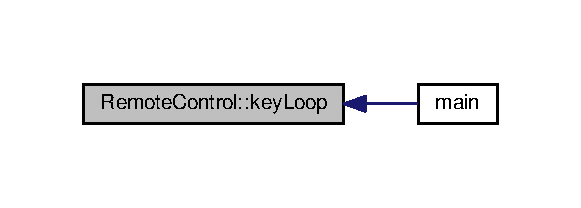
\includegraphics[width=279pt]{class_remote_control_afedba778e285038ada1cbcd9cb793502_icgraph}
\end{center}
\end{figure}




The documentation for this class was generated from the following file\+:\begin{DoxyCompactItemize}
\item 
/home/travis/build/\+Autonomous-\/\+Racing-\/\+P\+G/ros.\+package/docs/master/ros\+\_\+ws/src/auto\+\_\+race\+\_\+pg/src/\hyperlink{remote__control_8cpp}{remote\+\_\+control.\+cpp}\end{DoxyCompactItemize}

\hypertarget{class_remote_joy}{}\section{Remote\+Joy Class Reference}
\label{class_remote_joy}\index{Remote\+Joy@{Remote\+Joy}}
\subsection*{Public Member Functions}
\begin{DoxyCompactItemize}
\item 
\hyperlink{class_remote_joy_a88e2a07703d570a4b406c0a900c9493d}{Remote\+Joy} ()
\item 
void \hyperlink{class_remote_joy_aeb64e457c9661691877f98a7768473f7}{key\+Loop} ()
\end{DoxyCompactItemize}


\subsection{Detailed Description}


Definition at line 15 of file remote\+\_\+joy.\+cpp.



\subsection{Constructor \& Destructor Documentation}
\index{Remote\+Joy@{Remote\+Joy}!Remote\+Joy@{Remote\+Joy}}
\index{Remote\+Joy@{Remote\+Joy}!Remote\+Joy@{Remote\+Joy}}
\subsubsection[{\texorpdfstring{Remote\+Joy()}{RemoteJoy()}}]{\setlength{\rightskip}{0pt plus 5cm}Remote\+Joy\+::\+Remote\+Joy (
\begin{DoxyParamCaption}
{}
\end{DoxyParamCaption}
)}\hypertarget{class_remote_joy_a88e2a07703d570a4b406c0a900c9493d}{}\label{class_remote_joy_a88e2a07703d570a4b406c0a900c9493d}


Definition at line 37 of file remote\+\_\+joy.\+cpp.



\subsection{Member Function Documentation}
\index{Remote\+Joy@{Remote\+Joy}!key\+Loop@{key\+Loop}}
\index{key\+Loop@{key\+Loop}!Remote\+Joy@{Remote\+Joy}}
\subsubsection[{\texorpdfstring{key\+Loop()}{keyLoop()}}]{\setlength{\rightskip}{0pt plus 5cm}void Remote\+Joy\+::key\+Loop (
\begin{DoxyParamCaption}
{}
\end{DoxyParamCaption}
)}\hypertarget{class_remote_joy_aeb64e457c9661691877f98a7768473f7}{}\label{class_remote_joy_aeb64e457c9661691877f98a7768473f7}


The documentation for this class was generated from the following file\+:\begin{DoxyCompactItemize}
\item 
/home/travis/build/\+Autonomous-\/\+Racing-\/\+P\+G/ros.\+package/ros\+\_\+ws/src/auto\+\_\+race\+\_\+pg/src/\hyperlink{remote__joy_8cpp}{remote\+\_\+joy.\+cpp}\end{DoxyCompactItemize}

\hypertarget{class_remote_keyboard}{}\section{Remote\+Keyboard Class Reference}
\label{class_remote_keyboard}\index{Remote\+Keyboard@{Remote\+Keyboard}}


{\ttfamily \#include $<$remote\+\_\+keyboard.\+h$>$}

\subsection*{Public Member Functions}
\begin{DoxyCompactItemize}
\item 
\hyperlink{class_remote_keyboard_a95692cfc61f486ad020c47d49c1aca27}{Remote\+Keyboard} ()
\item 
void \hyperlink{class_remote_keyboard_a6e577da2cf6247e3cdbabd582784ba3c}{key\+Loop} ()
\end{DoxyCompactItemize}


\subsection{Detailed Description}


Definition at line 21 of file remote\+\_\+keyboard.\+h.



\subsection{Constructor \& Destructor Documentation}
\index{Remote\+Keyboard@{Remote\+Keyboard}!Remote\+Keyboard@{Remote\+Keyboard}}
\index{Remote\+Keyboard@{Remote\+Keyboard}!Remote\+Keyboard@{Remote\+Keyboard}}
\subsubsection[{\texorpdfstring{Remote\+Keyboard()}{RemoteKeyboard()}}]{\setlength{\rightskip}{0pt plus 5cm}Remote\+Keyboard\+::\+Remote\+Keyboard (
\begin{DoxyParamCaption}
{}
\end{DoxyParamCaption}
)}\hypertarget{class_remote_keyboard_a95692cfc61f486ad020c47d49c1aca27}{}\label{class_remote_keyboard_a95692cfc61f486ad020c47d49c1aca27}


Definition at line 3 of file remote\+\_\+keyboard.\+cpp.



\subsection{Member Function Documentation}
\index{Remote\+Keyboard@{Remote\+Keyboard}!key\+Loop@{key\+Loop}}
\index{key\+Loop@{key\+Loop}!Remote\+Keyboard@{Remote\+Keyboard}}
\subsubsection[{\texorpdfstring{key\+Loop()}{keyLoop()}}]{\setlength{\rightskip}{0pt plus 5cm}void Remote\+Keyboard\+::key\+Loop (
\begin{DoxyParamCaption}
{}
\end{DoxyParamCaption}
)}\hypertarget{class_remote_keyboard_a6e577da2cf6247e3cdbabd582784ba3c}{}\label{class_remote_keyboard_a6e577da2cf6247e3cdbabd582784ba3c}


Definition at line 11 of file remote\+\_\+keyboard.\+cpp.



Here is the caller graph for this function\+:
\nopagebreak
\begin{figure}[H]
\begin{center}
\leavevmode
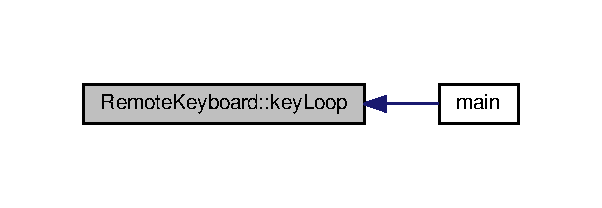
\includegraphics[width=289pt]{class_remote_keyboard_a6e577da2cf6247e3cdbabd582784ba3c_icgraph}
\end{center}
\end{figure}




The documentation for this class was generated from the following files\+:\begin{DoxyCompactItemize}
\item 
/home/travis/build/\+Autonomous-\/\+Racing-\/\+P\+G/ros.\+package/docs/master/ros\+\_\+ws/src/auto\+\_\+race\+\_\+pg/include/\hyperlink{remote__keyboard_8h}{remote\+\_\+keyboard.\+h}\item 
/home/travis/build/\+Autonomous-\/\+Racing-\/\+P\+G/ros.\+package/docs/master/ros\+\_\+ws/src/auto\+\_\+race\+\_\+pg/src/\hyperlink{remote__keyboard_8cpp}{remote\+\_\+keyboard.\+cpp}\end{DoxyCompactItemize}

\chapter{File Documentation}
\hypertarget{mainpage_8dox}{}\section{/home/travis/build/\+Autonomous-\/\+Racing-\/\+P\+G/ros.package/docs/master/doc/mainpage.dox File Reference}
\label{mainpage_8dox}\index{/home/travis/build/\+Autonomous-\/\+Racing-\/\+P\+G/ros.\+package/docs/master/doc/mainpage.\+dox@{/home/travis/build/\+Autonomous-\/\+Racing-\/\+P\+G/ros.\+package/docs/master/doc/mainpage.\+dox}}

\hypertarget{_r_e_a_d_m_e_8md}{}\section{/home/travis/build/\+Autonomous-\/\+Racing-\/\+P\+G/ros.package/\+R\+E\+A\+D\+ME.md File Reference}
\label{_r_e_a_d_m_e_8md}\index{/home/travis/build/\+Autonomous-\/\+Racing-\/\+P\+G/ros.\+package/\+R\+E\+A\+D\+M\+E.\+md@{/home/travis/build/\+Autonomous-\/\+Racing-\/\+P\+G/ros.\+package/\+R\+E\+A\+D\+M\+E.\+md}}

\hypertarget{car__control_8h}{}\section{/home/travis/build/\+Autonomous-\/\+Racing-\/\+P\+G/ros.package/docs/master/ros\+\_\+ws/src/car\+\_\+control/include/car\+\_\+control.h File Reference}
\label{car__control_8h}\index{/home/travis/build/\+Autonomous-\/\+Racing-\/\+P\+G/ros.\+package/docs/master/ros\+\_\+ws/src/car\+\_\+control/include/car\+\_\+control.\+h@{/home/travis/build/\+Autonomous-\/\+Racing-\/\+P\+G/ros.\+package/docs/master/ros\+\_\+ws/src/car\+\_\+control/include/car\+\_\+control.\+h}}
This graph shows which files directly or indirectly include this file\+:
\nopagebreak
\begin{figure}[H]
\begin{center}
\leavevmode
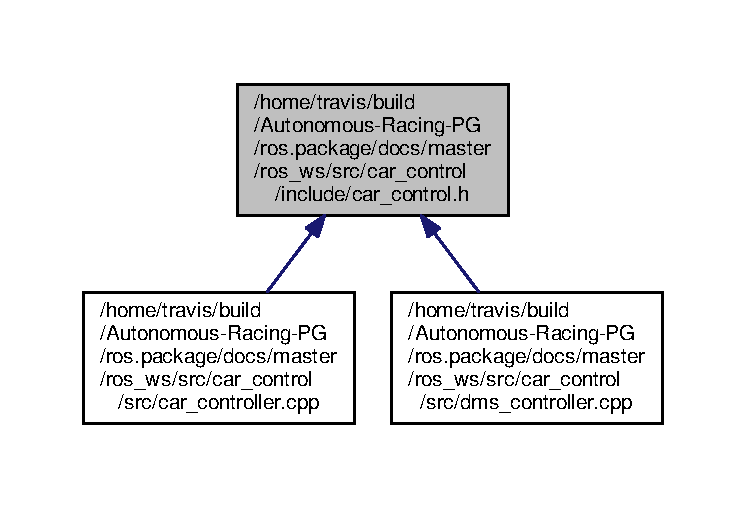
\includegraphics[width=350pt]{car__control_8h__dep__incl}
\end{center}
\end{figure}
\subsection*{Variables}
\begin{DoxyCompactItemize}
\item 
constexpr const char $\ast$ \hyperlink{car__control_8h_a6d4b6e4b84736143609cad22046a82fa}{C\+O\+M\+M\+A\+N\+D\+\_\+\+S\+T\+OP} = \char`\"{}stop\char`\"{}
\item 
constexpr const char $\ast$ \hyperlink{car__control_8h_a3ba962d8165c56ab8545410f4edd510f}{C\+O\+M\+M\+A\+N\+D\+\_\+\+GO} = \char`\"{}go\char`\"{}
\item 
constexpr const char $\ast$ \hyperlink{car__control_8h_a913c683c9209599c259aaebae91b557e}{T\+O\+P\+I\+C\+\_\+\+F\+O\+C\+B\+O\+X\+\_\+\+S\+P\+E\+ED} = \char`\"{}/commands/motor/speed\char`\"{}
\item 
constexpr const char $\ast$ \hyperlink{car__control_8h_a9fac7fea1c94a1d065ccd5b845ab45f7}{T\+O\+P\+I\+C\+\_\+\+F\+O\+C\+B\+O\+X\+\_\+\+A\+N\+G\+LE} = \char`\"{}/commands/servo/position\char`\"{}
\item 
constexpr const char $\ast$ \hyperlink{car__control_8h_a43c2621ae66c8cc9428026d680ed4fcb}{T\+O\+P\+I\+C\+\_\+\+F\+O\+C\+B\+O\+X\+\_\+\+B\+R\+A\+KE} = \char`\"{}commands/motor/brake\char`\"{}
\item 
constexpr const char $\ast$ \hyperlink{car__control_8h_ae2bdb9527cf2548c238295d766dcff5a}{T\+O\+P\+I\+C\+\_\+\+D\+R\+I\+V\+E\+\_\+\+P\+A\+R\+AM} = \char`\"{}/set/drive\+\_\+param\char`\"{}
\item 
constexpr const char $\ast$ \hyperlink{car__control_8h_a0f7f9cc9b6a6ff34aaf9f7acd8d3d044}{T\+O\+P\+I\+C\+\_\+\+C\+O\+M\+M\+A\+ND} = \char`\"{}/command\char`\"{}
\item 
constexpr const char $\ast$ \hyperlink{car__control_8h_a1e56417499d1048f130bc194015c7bef}{T\+O\+P\+I\+C\+\_\+\+D\+MS} = \char`\"{}/set/dms\char`\"{}
\end{DoxyCompactItemize}


\subsection{Variable Documentation}
\index{car\+\_\+control.\+h@{car\+\_\+control.\+h}!C\+O\+M\+M\+A\+N\+D\+\_\+\+GO@{C\+O\+M\+M\+A\+N\+D\+\_\+\+GO}}
\index{C\+O\+M\+M\+A\+N\+D\+\_\+\+GO@{C\+O\+M\+M\+A\+N\+D\+\_\+\+GO}!car\+\_\+control.\+h@{car\+\_\+control.\+h}}
\subsubsection[{\texorpdfstring{C\+O\+M\+M\+A\+N\+D\+\_\+\+GO}{COMMAND_GO}}]{\setlength{\rightskip}{0pt plus 5cm}constexpr const char$\ast$ C\+O\+M\+M\+A\+N\+D\+\_\+\+GO = \char`\"{}go\char`\"{}}\hypertarget{car__control_8h_a3ba962d8165c56ab8545410f4edd510f}{}\label{car__control_8h_a3ba962d8165c56ab8545410f4edd510f}


Definition at line 5 of file car\+\_\+control.\+h.

\index{car\+\_\+control.\+h@{car\+\_\+control.\+h}!C\+O\+M\+M\+A\+N\+D\+\_\+\+S\+T\+OP@{C\+O\+M\+M\+A\+N\+D\+\_\+\+S\+T\+OP}}
\index{C\+O\+M\+M\+A\+N\+D\+\_\+\+S\+T\+OP@{C\+O\+M\+M\+A\+N\+D\+\_\+\+S\+T\+OP}!car\+\_\+control.\+h@{car\+\_\+control.\+h}}
\subsubsection[{\texorpdfstring{C\+O\+M\+M\+A\+N\+D\+\_\+\+S\+T\+OP}{COMMAND_STOP}}]{\setlength{\rightskip}{0pt plus 5cm}constexpr const char$\ast$ C\+O\+M\+M\+A\+N\+D\+\_\+\+S\+T\+OP = \char`\"{}stop\char`\"{}}\hypertarget{car__control_8h_a6d4b6e4b84736143609cad22046a82fa}{}\label{car__control_8h_a6d4b6e4b84736143609cad22046a82fa}


Definition at line 4 of file car\+\_\+control.\+h.

\index{car\+\_\+control.\+h@{car\+\_\+control.\+h}!T\+O\+P\+I\+C\+\_\+\+C\+O\+M\+M\+A\+ND@{T\+O\+P\+I\+C\+\_\+\+C\+O\+M\+M\+A\+ND}}
\index{T\+O\+P\+I\+C\+\_\+\+C\+O\+M\+M\+A\+ND@{T\+O\+P\+I\+C\+\_\+\+C\+O\+M\+M\+A\+ND}!car\+\_\+control.\+h@{car\+\_\+control.\+h}}
\subsubsection[{\texorpdfstring{T\+O\+P\+I\+C\+\_\+\+C\+O\+M\+M\+A\+ND}{TOPIC_COMMAND}}]{\setlength{\rightskip}{0pt plus 5cm}constexpr const char$\ast$ T\+O\+P\+I\+C\+\_\+\+C\+O\+M\+M\+A\+ND = \char`\"{}/command\char`\"{}}\hypertarget{car__control_8h_a0f7f9cc9b6a6ff34aaf9f7acd8d3d044}{}\label{car__control_8h_a0f7f9cc9b6a6ff34aaf9f7acd8d3d044}


Definition at line 13 of file car\+\_\+control.\+h.

\index{car\+\_\+control.\+h@{car\+\_\+control.\+h}!T\+O\+P\+I\+C\+\_\+\+D\+MS@{T\+O\+P\+I\+C\+\_\+\+D\+MS}}
\index{T\+O\+P\+I\+C\+\_\+\+D\+MS@{T\+O\+P\+I\+C\+\_\+\+D\+MS}!car\+\_\+control.\+h@{car\+\_\+control.\+h}}
\subsubsection[{\texorpdfstring{T\+O\+P\+I\+C\+\_\+\+D\+MS}{TOPIC_DMS}}]{\setlength{\rightskip}{0pt plus 5cm}constexpr const char$\ast$ T\+O\+P\+I\+C\+\_\+\+D\+MS = \char`\"{}/set/dms\char`\"{}}\hypertarget{car__control_8h_a1e56417499d1048f130bc194015c7bef}{}\label{car__control_8h_a1e56417499d1048f130bc194015c7bef}


Definition at line 14 of file car\+\_\+control.\+h.

\index{car\+\_\+control.\+h@{car\+\_\+control.\+h}!T\+O\+P\+I\+C\+\_\+\+D\+R\+I\+V\+E\+\_\+\+P\+A\+R\+AM@{T\+O\+P\+I\+C\+\_\+\+D\+R\+I\+V\+E\+\_\+\+P\+A\+R\+AM}}
\index{T\+O\+P\+I\+C\+\_\+\+D\+R\+I\+V\+E\+\_\+\+P\+A\+R\+AM@{T\+O\+P\+I\+C\+\_\+\+D\+R\+I\+V\+E\+\_\+\+P\+A\+R\+AM}!car\+\_\+control.\+h@{car\+\_\+control.\+h}}
\subsubsection[{\texorpdfstring{T\+O\+P\+I\+C\+\_\+\+D\+R\+I\+V\+E\+\_\+\+P\+A\+R\+AM}{TOPIC_DRIVE_PARAM}}]{\setlength{\rightskip}{0pt plus 5cm}constexpr const char$\ast$ T\+O\+P\+I\+C\+\_\+\+D\+R\+I\+V\+E\+\_\+\+P\+A\+R\+AM = \char`\"{}/set/drive\+\_\+param\char`\"{}}\hypertarget{car__control_8h_ae2bdb9527cf2548c238295d766dcff5a}{}\label{car__control_8h_ae2bdb9527cf2548c238295d766dcff5a}


Definition at line 12 of file car\+\_\+control.\+h.

\index{car\+\_\+control.\+h@{car\+\_\+control.\+h}!T\+O\+P\+I\+C\+\_\+\+F\+O\+C\+B\+O\+X\+\_\+\+A\+N\+G\+LE@{T\+O\+P\+I\+C\+\_\+\+F\+O\+C\+B\+O\+X\+\_\+\+A\+N\+G\+LE}}
\index{T\+O\+P\+I\+C\+\_\+\+F\+O\+C\+B\+O\+X\+\_\+\+A\+N\+G\+LE@{T\+O\+P\+I\+C\+\_\+\+F\+O\+C\+B\+O\+X\+\_\+\+A\+N\+G\+LE}!car\+\_\+control.\+h@{car\+\_\+control.\+h}}
\subsubsection[{\texorpdfstring{T\+O\+P\+I\+C\+\_\+\+F\+O\+C\+B\+O\+X\+\_\+\+A\+N\+G\+LE}{TOPIC_FOCBOX_ANGLE}}]{\setlength{\rightskip}{0pt plus 5cm}constexpr const char$\ast$ T\+O\+P\+I\+C\+\_\+\+F\+O\+C\+B\+O\+X\+\_\+\+A\+N\+G\+LE = \char`\"{}/commands/servo/position\char`\"{}}\hypertarget{car__control_8h_a9fac7fea1c94a1d065ccd5b845ab45f7}{}\label{car__control_8h_a9fac7fea1c94a1d065ccd5b845ab45f7}


Definition at line 9 of file car\+\_\+control.\+h.

\index{car\+\_\+control.\+h@{car\+\_\+control.\+h}!T\+O\+P\+I\+C\+\_\+\+F\+O\+C\+B\+O\+X\+\_\+\+B\+R\+A\+KE@{T\+O\+P\+I\+C\+\_\+\+F\+O\+C\+B\+O\+X\+\_\+\+B\+R\+A\+KE}}
\index{T\+O\+P\+I\+C\+\_\+\+F\+O\+C\+B\+O\+X\+\_\+\+B\+R\+A\+KE@{T\+O\+P\+I\+C\+\_\+\+F\+O\+C\+B\+O\+X\+\_\+\+B\+R\+A\+KE}!car\+\_\+control.\+h@{car\+\_\+control.\+h}}
\subsubsection[{\texorpdfstring{T\+O\+P\+I\+C\+\_\+\+F\+O\+C\+B\+O\+X\+\_\+\+B\+R\+A\+KE}{TOPIC_FOCBOX_BRAKE}}]{\setlength{\rightskip}{0pt plus 5cm}constexpr const char$\ast$ T\+O\+P\+I\+C\+\_\+\+F\+O\+C\+B\+O\+X\+\_\+\+B\+R\+A\+KE = \char`\"{}commands/motor/brake\char`\"{}}\hypertarget{car__control_8h_a43c2621ae66c8cc9428026d680ed4fcb}{}\label{car__control_8h_a43c2621ae66c8cc9428026d680ed4fcb}


Definition at line 10 of file car\+\_\+control.\+h.

\index{car\+\_\+control.\+h@{car\+\_\+control.\+h}!T\+O\+P\+I\+C\+\_\+\+F\+O\+C\+B\+O\+X\+\_\+\+S\+P\+E\+ED@{T\+O\+P\+I\+C\+\_\+\+F\+O\+C\+B\+O\+X\+\_\+\+S\+P\+E\+ED}}
\index{T\+O\+P\+I\+C\+\_\+\+F\+O\+C\+B\+O\+X\+\_\+\+S\+P\+E\+ED@{T\+O\+P\+I\+C\+\_\+\+F\+O\+C\+B\+O\+X\+\_\+\+S\+P\+E\+ED}!car\+\_\+control.\+h@{car\+\_\+control.\+h}}
\subsubsection[{\texorpdfstring{T\+O\+P\+I\+C\+\_\+\+F\+O\+C\+B\+O\+X\+\_\+\+S\+P\+E\+ED}{TOPIC_FOCBOX_SPEED}}]{\setlength{\rightskip}{0pt plus 5cm}constexpr const char$\ast$ T\+O\+P\+I\+C\+\_\+\+F\+O\+C\+B\+O\+X\+\_\+\+S\+P\+E\+ED = \char`\"{}/commands/motor/speed\char`\"{}}\hypertarget{car__control_8h_a913c683c9209599c259aaebae91b557e}{}\label{car__control_8h_a913c683c9209599c259aaebae91b557e}


Definition at line 8 of file car\+\_\+control.\+h.


\hypertarget{remote__joy_8h}{}\section{/home/travis/build/\+Autonomous-\/\+Racing-\/\+P\+G/ros.package/docs/master/ros\+\_\+ws/src/auto\+\_\+race\+\_\+pg/include/remote\+\_\+joy.h File Reference}
\label{remote__joy_8h}\index{/home/travis/build/\+Autonomous-\/\+Racing-\/\+P\+G/ros.\+package/docs/master/ros\+\_\+ws/src/auto\+\_\+race\+\_\+pg/include/remote\+\_\+joy.\+h@{/home/travis/build/\+Autonomous-\/\+Racing-\/\+P\+G/ros.\+package/docs/master/ros\+\_\+ws/src/auto\+\_\+race\+\_\+pg/include/remote\+\_\+joy.\+h}}
{\ttfamily \#include $<$ros/ros.\+h$>$}\\*
{\ttfamily \#include $<$sensor\+\_\+msgs/\+Joy.\+h$>$}\\*
{\ttfamily \#include $<$std\+\_\+msgs/\+Float64.\+h$>$}\\*
Include dependency graph for remote\+\_\+joy.\+h\+:
\nopagebreak
\begin{figure}[H]
\begin{center}
\leavevmode
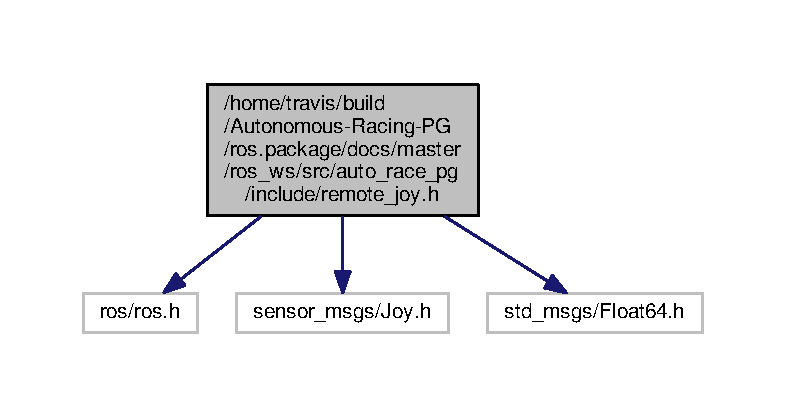
\includegraphics[width=350pt]{remote__joy_8h__incl}
\end{center}
\end{figure}
This graph shows which files directly or indirectly include this file\+:
\nopagebreak
\begin{figure}[H]
\begin{center}
\leavevmode
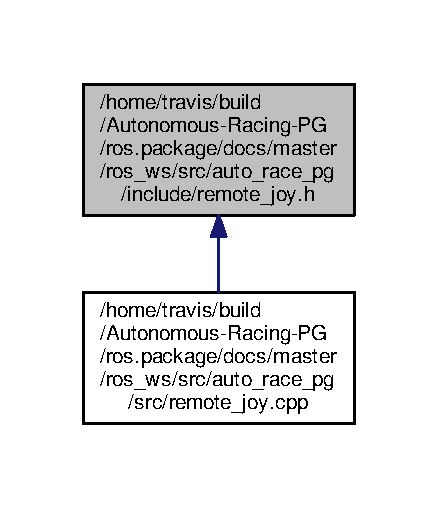
\includegraphics[width=210pt]{remote__joy_8h__dep__incl}
\end{center}
\end{figure}
\subsection*{Classes}
\begin{DoxyCompactItemize}
\item 
class \hyperlink{class_remote_joy}{Remote\+Joy}
\end{DoxyCompactItemize}
\subsection*{Macros}
\begin{DoxyCompactItemize}
\item 
\#define \hyperlink{remote__joy_8h_af31f8d44964078052dd8e23754b320c8}{M\+A\+X\+\_\+\+R\+E\+V\+E\+R\+S\+E\+\_\+\+S\+P\+E\+ED}~0.\+1
\item 
\#define \hyperlink{remote__joy_8h_acbfb5eae88329444b807a7b3a180d855}{J\+O\+Y\+\_\+\+A\+N\+G\+L\+E\+\_\+\+A\+N\+G\+U\+L\+AR}~0
\item 
\#define \hyperlink{remote__joy_8h_a447fc4cb069a0478754727f0383f7e1b}{J\+O\+Y\+\_\+\+A\+N\+G\+L\+E\+\_\+\+L\+I\+N\+E\+AR}~1
\item 
\#define \hyperlink{remote__joy_8h_ab792c1a92e80d836749be62819b376d9}{J\+O\+Y\+\_\+\+R2}~2
\item 
\#define \hyperlink{remote__joy_8h_a8c6b7fe5ad62f0dd9be385ca98ca1c9a}{T\+O\+P\+I\+C\+\_\+\+S\+P\+E\+ED}~\char`\"{}/set/speed\char`\"{}
\item 
\#define \hyperlink{remote__joy_8h_ae85d82183138111cc259bc2920f54e9f}{T\+O\+P\+I\+C\+\_\+\+A\+N\+G\+LE}~\char`\"{}/set/angle\char`\"{}
\end{DoxyCompactItemize}


\subsection{Macro Definition Documentation}
\index{remote\+\_\+joy.\+h@{remote\+\_\+joy.\+h}!J\+O\+Y\+\_\+\+A\+N\+G\+L\+E\+\_\+\+A\+N\+G\+U\+L\+AR@{J\+O\+Y\+\_\+\+A\+N\+G\+L\+E\+\_\+\+A\+N\+G\+U\+L\+AR}}
\index{J\+O\+Y\+\_\+\+A\+N\+G\+L\+E\+\_\+\+A\+N\+G\+U\+L\+AR@{J\+O\+Y\+\_\+\+A\+N\+G\+L\+E\+\_\+\+A\+N\+G\+U\+L\+AR}!remote\+\_\+joy.\+h@{remote\+\_\+joy.\+h}}
\subsubsection[{\texorpdfstring{J\+O\+Y\+\_\+\+A\+N\+G\+L\+E\+\_\+\+A\+N\+G\+U\+L\+AR}{JOY_ANGLE_ANGULAR}}]{\setlength{\rightskip}{0pt plus 5cm}\#define J\+O\+Y\+\_\+\+A\+N\+G\+L\+E\+\_\+\+A\+N\+G\+U\+L\+AR~0}\hypertarget{remote__joy_8h_acbfb5eae88329444b807a7b3a180d855}{}\label{remote__joy_8h_acbfb5eae88329444b807a7b3a180d855}


Definition at line 10 of file remote\+\_\+joy.\+h.

\index{remote\+\_\+joy.\+h@{remote\+\_\+joy.\+h}!J\+O\+Y\+\_\+\+A\+N\+G\+L\+E\+\_\+\+L\+I\+N\+E\+AR@{J\+O\+Y\+\_\+\+A\+N\+G\+L\+E\+\_\+\+L\+I\+N\+E\+AR}}
\index{J\+O\+Y\+\_\+\+A\+N\+G\+L\+E\+\_\+\+L\+I\+N\+E\+AR@{J\+O\+Y\+\_\+\+A\+N\+G\+L\+E\+\_\+\+L\+I\+N\+E\+AR}!remote\+\_\+joy.\+h@{remote\+\_\+joy.\+h}}
\subsubsection[{\texorpdfstring{J\+O\+Y\+\_\+\+A\+N\+G\+L\+E\+\_\+\+L\+I\+N\+E\+AR}{JOY_ANGLE_LINEAR}}]{\setlength{\rightskip}{0pt plus 5cm}\#define J\+O\+Y\+\_\+\+A\+N\+G\+L\+E\+\_\+\+L\+I\+N\+E\+AR~1}\hypertarget{remote__joy_8h_a447fc4cb069a0478754727f0383f7e1b}{}\label{remote__joy_8h_a447fc4cb069a0478754727f0383f7e1b}


Definition at line 11 of file remote\+\_\+joy.\+h.

\index{remote\+\_\+joy.\+h@{remote\+\_\+joy.\+h}!J\+O\+Y\+\_\+\+R2@{J\+O\+Y\+\_\+\+R2}}
\index{J\+O\+Y\+\_\+\+R2@{J\+O\+Y\+\_\+\+R2}!remote\+\_\+joy.\+h@{remote\+\_\+joy.\+h}}
\subsubsection[{\texorpdfstring{J\+O\+Y\+\_\+\+R2}{JOY_R2}}]{\setlength{\rightskip}{0pt plus 5cm}\#define J\+O\+Y\+\_\+\+R2~2}\hypertarget{remote__joy_8h_ab792c1a92e80d836749be62819b376d9}{}\label{remote__joy_8h_ab792c1a92e80d836749be62819b376d9}


Definition at line 12 of file remote\+\_\+joy.\+h.

\index{remote\+\_\+joy.\+h@{remote\+\_\+joy.\+h}!M\+A\+X\+\_\+\+R\+E\+V\+E\+R\+S\+E\+\_\+\+S\+P\+E\+ED@{M\+A\+X\+\_\+\+R\+E\+V\+E\+R\+S\+E\+\_\+\+S\+P\+E\+ED}}
\index{M\+A\+X\+\_\+\+R\+E\+V\+E\+R\+S\+E\+\_\+\+S\+P\+E\+ED@{M\+A\+X\+\_\+\+R\+E\+V\+E\+R\+S\+E\+\_\+\+S\+P\+E\+ED}!remote\+\_\+joy.\+h@{remote\+\_\+joy.\+h}}
\subsubsection[{\texorpdfstring{M\+A\+X\+\_\+\+R\+E\+V\+E\+R\+S\+E\+\_\+\+S\+P\+E\+ED}{MAX_REVERSE_SPEED}}]{\setlength{\rightskip}{0pt plus 5cm}\#define M\+A\+X\+\_\+\+R\+E\+V\+E\+R\+S\+E\+\_\+\+S\+P\+E\+ED~0.\+1}\hypertarget{remote__joy_8h_af31f8d44964078052dd8e23754b320c8}{}\label{remote__joy_8h_af31f8d44964078052dd8e23754b320c8}


Definition at line 8 of file remote\+\_\+joy.\+h.

\index{remote\+\_\+joy.\+h@{remote\+\_\+joy.\+h}!T\+O\+P\+I\+C\+\_\+\+A\+N\+G\+LE@{T\+O\+P\+I\+C\+\_\+\+A\+N\+G\+LE}}
\index{T\+O\+P\+I\+C\+\_\+\+A\+N\+G\+LE@{T\+O\+P\+I\+C\+\_\+\+A\+N\+G\+LE}!remote\+\_\+joy.\+h@{remote\+\_\+joy.\+h}}
\subsubsection[{\texorpdfstring{T\+O\+P\+I\+C\+\_\+\+A\+N\+G\+LE}{TOPIC_ANGLE}}]{\setlength{\rightskip}{0pt plus 5cm}\#define T\+O\+P\+I\+C\+\_\+\+A\+N\+G\+LE~\char`\"{}/set/angle\char`\"{}}\hypertarget{remote__joy_8h_ae85d82183138111cc259bc2920f54e9f}{}\label{remote__joy_8h_ae85d82183138111cc259bc2920f54e9f}


Definition at line 15 of file remote\+\_\+joy.\+h.

\index{remote\+\_\+joy.\+h@{remote\+\_\+joy.\+h}!T\+O\+P\+I\+C\+\_\+\+S\+P\+E\+ED@{T\+O\+P\+I\+C\+\_\+\+S\+P\+E\+ED}}
\index{T\+O\+P\+I\+C\+\_\+\+S\+P\+E\+ED@{T\+O\+P\+I\+C\+\_\+\+S\+P\+E\+ED}!remote\+\_\+joy.\+h@{remote\+\_\+joy.\+h}}
\subsubsection[{\texorpdfstring{T\+O\+P\+I\+C\+\_\+\+S\+P\+E\+ED}{TOPIC_SPEED}}]{\setlength{\rightskip}{0pt plus 5cm}\#define T\+O\+P\+I\+C\+\_\+\+S\+P\+E\+ED~\char`\"{}/set/speed\char`\"{}}\hypertarget{remote__joy_8h_a8c6b7fe5ad62f0dd9be385ca98ca1c9a}{}\label{remote__joy_8h_a8c6b7fe5ad62f0dd9be385ca98ca1c9a}


Definition at line 14 of file remote\+\_\+joy.\+h.


\hypertarget{remote__keyboard_8h}{}\section{/home/travis/build/\+Autonomous-\/\+Racing-\/\+P\+G/ros.package/docs/master/ros\+\_\+ws/src/auto\+\_\+race\+\_\+pg/include/remote\+\_\+keyboard.h File Reference}
\label{remote__keyboard_8h}\index{/home/travis/build/\+Autonomous-\/\+Racing-\/\+P\+G/ros.\+package/docs/master/ros\+\_\+ws/src/auto\+\_\+race\+\_\+pg/include/remote\+\_\+keyboard.\+h@{/home/travis/build/\+Autonomous-\/\+Racing-\/\+P\+G/ros.\+package/docs/master/ros\+\_\+ws/src/auto\+\_\+race\+\_\+pg/include/remote\+\_\+keyboard.\+h}}
{\ttfamily \#include $<$ros/ros.\+h$>$}\\*
{\ttfamily \#include $<$std\+\_\+msgs/\+Float64.\+h$>$}\\*
{\ttfamily \#include $<$std\+\_\+msgs/\+Int64.\+h$>$}\\*
{\ttfamily \#include $<$signal.\+h$>$}\\*
{\ttfamily \#include $<$termios.\+h$>$}\\*
{\ttfamily \#include $<$time.\+h$>$}\\*
Include dependency graph for remote\+\_\+keyboard.\+h\+:
\nopagebreak
\begin{figure}[H]
\begin{center}
\leavevmode
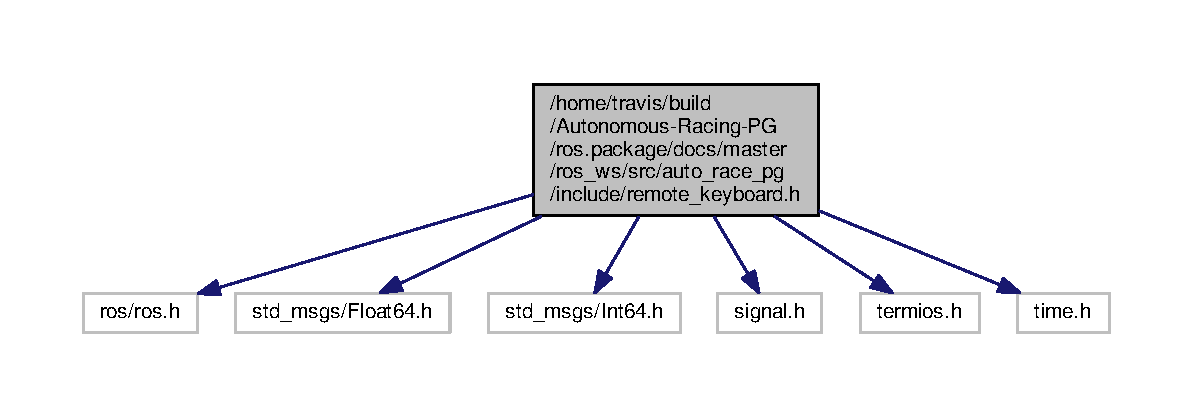
\includegraphics[width=350pt]{remote__keyboard_8h__incl}
\end{center}
\end{figure}
This graph shows which files directly or indirectly include this file\+:
\nopagebreak
\begin{figure}[H]
\begin{center}
\leavevmode
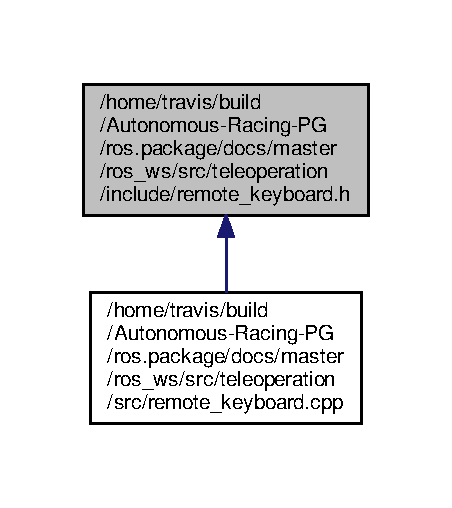
\includegraphics[width=217pt]{remote__keyboard_8h__dep__incl}
\end{center}
\end{figure}
\subsection*{Classes}
\begin{DoxyCompactItemize}
\item 
class \hyperlink{class_remote_keyboard}{Remote\+Keyboard}
\end{DoxyCompactItemize}
\subsection*{Macros}
\begin{DoxyCompactItemize}
\item 
\#define \hyperlink{remote__keyboard_8h_a8c6b7fe5ad62f0dd9be385ca98ca1c9a}{T\+O\+P\+I\+C\+\_\+\+S\+P\+E\+ED}~\char`\"{}/set/speed\char`\"{}
\item 
\#define \hyperlink{remote__keyboard_8h_ae85d82183138111cc259bc2920f54e9f}{T\+O\+P\+I\+C\+\_\+\+A\+N\+G\+LE}~\char`\"{}/set/angle\char`\"{}
\item 
\#define \hyperlink{remote__keyboard_8h_a6a44fd7e61a3f73fffecd1ec5973f819}{K\+E\+Y\+C\+O\+D\+E\+\_\+W}~119
\item 
\#define \hyperlink{remote__keyboard_8h_a35ba55030dedad2411239e6330435742}{K\+E\+Y\+C\+O\+D\+E\+\_\+A}~97
\item 
\#define \hyperlink{remote__keyboard_8h_a9be3d5563fec0f900d20668973b5806c}{K\+E\+Y\+C\+O\+D\+E\+\_\+S}~115
\item 
\#define \hyperlink{remote__keyboard_8h_af0c998786dcada98bf809fea0b157603}{K\+E\+Y\+C\+O\+D\+E\+\_\+D}~100
\item 
\#define \hyperlink{remote__keyboard_8h_a49115085a0fac000fb82c9d86c4c34d3}{K\+E\+Y\+C\+O\+D\+E\+\_\+\+S\+P\+A\+CE}~32
\end{DoxyCompactItemize}


\subsection{Macro Definition Documentation}
\index{remote\+\_\+keyboard.\+h@{remote\+\_\+keyboard.\+h}!K\+E\+Y\+C\+O\+D\+E\+\_\+A@{K\+E\+Y\+C\+O\+D\+E\+\_\+A}}
\index{K\+E\+Y\+C\+O\+D\+E\+\_\+A@{K\+E\+Y\+C\+O\+D\+E\+\_\+A}!remote\+\_\+keyboard.\+h@{remote\+\_\+keyboard.\+h}}
\subsubsection[{\texorpdfstring{K\+E\+Y\+C\+O\+D\+E\+\_\+A}{KEYCODE_A}}]{\setlength{\rightskip}{0pt plus 5cm}\#define K\+E\+Y\+C\+O\+D\+E\+\_\+A~97}\hypertarget{remote__keyboard_8h_a35ba55030dedad2411239e6330435742}{}\label{remote__keyboard_8h_a35ba55030dedad2411239e6330435742}


Definition at line 16 of file remote\+\_\+keyboard.\+h.

\index{remote\+\_\+keyboard.\+h@{remote\+\_\+keyboard.\+h}!K\+E\+Y\+C\+O\+D\+E\+\_\+D@{K\+E\+Y\+C\+O\+D\+E\+\_\+D}}
\index{K\+E\+Y\+C\+O\+D\+E\+\_\+D@{K\+E\+Y\+C\+O\+D\+E\+\_\+D}!remote\+\_\+keyboard.\+h@{remote\+\_\+keyboard.\+h}}
\subsubsection[{\texorpdfstring{K\+E\+Y\+C\+O\+D\+E\+\_\+D}{KEYCODE_D}}]{\setlength{\rightskip}{0pt plus 5cm}\#define K\+E\+Y\+C\+O\+D\+E\+\_\+D~100}\hypertarget{remote__keyboard_8h_af0c998786dcada98bf809fea0b157603}{}\label{remote__keyboard_8h_af0c998786dcada98bf809fea0b157603}


Definition at line 18 of file remote\+\_\+keyboard.\+h.

\index{remote\+\_\+keyboard.\+h@{remote\+\_\+keyboard.\+h}!K\+E\+Y\+C\+O\+D\+E\+\_\+S@{K\+E\+Y\+C\+O\+D\+E\+\_\+S}}
\index{K\+E\+Y\+C\+O\+D\+E\+\_\+S@{K\+E\+Y\+C\+O\+D\+E\+\_\+S}!remote\+\_\+keyboard.\+h@{remote\+\_\+keyboard.\+h}}
\subsubsection[{\texorpdfstring{K\+E\+Y\+C\+O\+D\+E\+\_\+S}{KEYCODE_S}}]{\setlength{\rightskip}{0pt plus 5cm}\#define K\+E\+Y\+C\+O\+D\+E\+\_\+S~115}\hypertarget{remote__keyboard_8h_a9be3d5563fec0f900d20668973b5806c}{}\label{remote__keyboard_8h_a9be3d5563fec0f900d20668973b5806c}


Definition at line 17 of file remote\+\_\+keyboard.\+h.

\index{remote\+\_\+keyboard.\+h@{remote\+\_\+keyboard.\+h}!K\+E\+Y\+C\+O\+D\+E\+\_\+\+S\+P\+A\+CE@{K\+E\+Y\+C\+O\+D\+E\+\_\+\+S\+P\+A\+CE}}
\index{K\+E\+Y\+C\+O\+D\+E\+\_\+\+S\+P\+A\+CE@{K\+E\+Y\+C\+O\+D\+E\+\_\+\+S\+P\+A\+CE}!remote\+\_\+keyboard.\+h@{remote\+\_\+keyboard.\+h}}
\subsubsection[{\texorpdfstring{K\+E\+Y\+C\+O\+D\+E\+\_\+\+S\+P\+A\+CE}{KEYCODE_SPACE}}]{\setlength{\rightskip}{0pt plus 5cm}\#define K\+E\+Y\+C\+O\+D\+E\+\_\+\+S\+P\+A\+CE~32}\hypertarget{remote__keyboard_8h_a49115085a0fac000fb82c9d86c4c34d3}{}\label{remote__keyboard_8h_a49115085a0fac000fb82c9d86c4c34d3}


Definition at line 19 of file remote\+\_\+keyboard.\+h.

\index{remote\+\_\+keyboard.\+h@{remote\+\_\+keyboard.\+h}!K\+E\+Y\+C\+O\+D\+E\+\_\+W@{K\+E\+Y\+C\+O\+D\+E\+\_\+W}}
\index{K\+E\+Y\+C\+O\+D\+E\+\_\+W@{K\+E\+Y\+C\+O\+D\+E\+\_\+W}!remote\+\_\+keyboard.\+h@{remote\+\_\+keyboard.\+h}}
\subsubsection[{\texorpdfstring{K\+E\+Y\+C\+O\+D\+E\+\_\+W}{KEYCODE_W}}]{\setlength{\rightskip}{0pt plus 5cm}\#define K\+E\+Y\+C\+O\+D\+E\+\_\+W~119}\hypertarget{remote__keyboard_8h_a6a44fd7e61a3f73fffecd1ec5973f819}{}\label{remote__keyboard_8h_a6a44fd7e61a3f73fffecd1ec5973f819}


Definition at line 15 of file remote\+\_\+keyboard.\+h.

\index{remote\+\_\+keyboard.\+h@{remote\+\_\+keyboard.\+h}!T\+O\+P\+I\+C\+\_\+\+A\+N\+G\+LE@{T\+O\+P\+I\+C\+\_\+\+A\+N\+G\+LE}}
\index{T\+O\+P\+I\+C\+\_\+\+A\+N\+G\+LE@{T\+O\+P\+I\+C\+\_\+\+A\+N\+G\+LE}!remote\+\_\+keyboard.\+h@{remote\+\_\+keyboard.\+h}}
\subsubsection[{\texorpdfstring{T\+O\+P\+I\+C\+\_\+\+A\+N\+G\+LE}{TOPIC_ANGLE}}]{\setlength{\rightskip}{0pt plus 5cm}\#define T\+O\+P\+I\+C\+\_\+\+A\+N\+G\+LE~\char`\"{}/set/angle\char`\"{}}\hypertarget{remote__keyboard_8h_ae85d82183138111cc259bc2920f54e9f}{}\label{remote__keyboard_8h_ae85d82183138111cc259bc2920f54e9f}


Definition at line 13 of file remote\+\_\+keyboard.\+h.

\index{remote\+\_\+keyboard.\+h@{remote\+\_\+keyboard.\+h}!T\+O\+P\+I\+C\+\_\+\+S\+P\+E\+ED@{T\+O\+P\+I\+C\+\_\+\+S\+P\+E\+ED}}
\index{T\+O\+P\+I\+C\+\_\+\+S\+P\+E\+ED@{T\+O\+P\+I\+C\+\_\+\+S\+P\+E\+ED}!remote\+\_\+keyboard.\+h@{remote\+\_\+keyboard.\+h}}
\subsubsection[{\texorpdfstring{T\+O\+P\+I\+C\+\_\+\+S\+P\+E\+ED}{TOPIC_SPEED}}]{\setlength{\rightskip}{0pt plus 5cm}\#define T\+O\+P\+I\+C\+\_\+\+S\+P\+E\+ED~\char`\"{}/set/speed\char`\"{}}\hypertarget{remote__keyboard_8h_a8c6b7fe5ad62f0dd9be385ca98ca1c9a}{}\label{remote__keyboard_8h_a8c6b7fe5ad62f0dd9be385ca98ca1c9a}


Definition at line 12 of file remote\+\_\+keyboard.\+h.


\hypertarget{car__control_8cpp}{}\section{/home/travis/build/\+Autonomous-\/\+Racing-\/\+P\+G/ros.package/ros\+\_\+ws/src/auto\+\_\+race\+\_\+pg/src/car\+\_\+control.cpp File Reference}
\label{car__control_8cpp}\index{/home/travis/build/\+Autonomous-\/\+Racing-\/\+P\+G/ros.\+package/ros\+\_\+ws/src/auto\+\_\+race\+\_\+pg/src/car\+\_\+control.\+cpp@{/home/travis/build/\+Autonomous-\/\+Racing-\/\+P\+G/ros.\+package/ros\+\_\+ws/src/auto\+\_\+race\+\_\+pg/src/car\+\_\+control.\+cpp}}
{\ttfamily \#include $<$ros/ros.\+h$>$}\\*
{\ttfamily \#include $<$time.\+h$>$}\\*
{\ttfamily \#include $<$std\+\_\+msgs/\+Float64.\+h$>$}\\*
{\ttfamily \#include $<$std\+\_\+msgs/\+String.\+h$>$}\\*
{\ttfamily \#include $<$std\+\_\+msgs/\+Int64.\+h$>$}\\*
Include dependency graph for car\+\_\+control.\+cpp\+:
\nopagebreak
\begin{figure}[H]
\begin{center}
\leavevmode
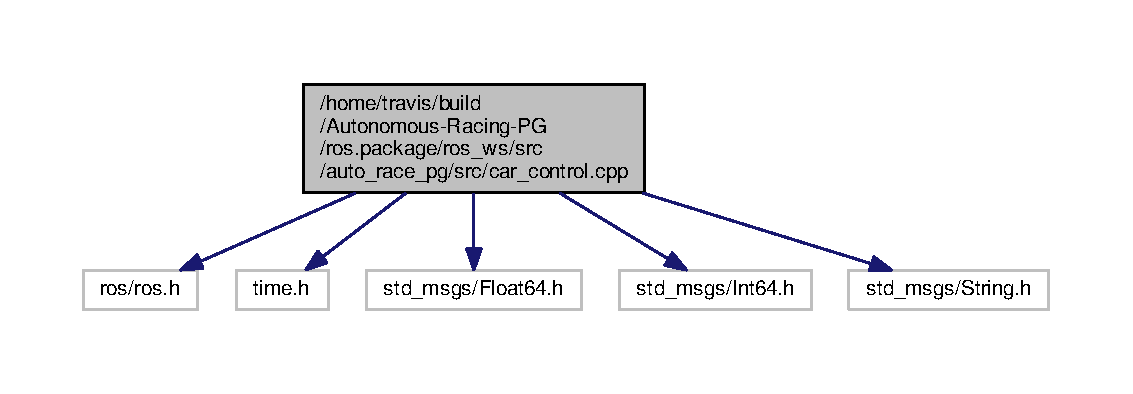
\includegraphics[width=350pt]{car__control_8cpp__incl}
\end{center}
\end{figure}
\subsection*{Classes}
\begin{DoxyCompactItemize}
\item 
class \hyperlink{class_car_control}{Car\+Control}
\end{DoxyCompactItemize}
\subsection*{Macros}
\begin{DoxyCompactItemize}
\item 
\#define \hyperlink{car__control_8cpp_a6977f30ada15874c2885ecd86dab7bd1}{T\+O\+P\+I\+C\+\_\+\+F\+O\+C\+B\+O\+X\+\_\+\+S\+P\+E\+ED}~\char`\"{}/commands/motor/speed\char`\"{}
\item 
\#define \hyperlink{car__control_8cpp_a06bf2e121cdcd87f3e73500ff616ccf2}{T\+O\+P\+I\+C\+\_\+\+F\+O\+C\+B\+O\+X\+\_\+\+A\+N\+G\+LE}~\char`\"{}/commands/servo/position\char`\"{}
\item 
\#define \hyperlink{car__control_8cpp_a8c6b7fe5ad62f0dd9be385ca98ca1c9a}{T\+O\+P\+I\+C\+\_\+\+S\+P\+E\+ED}~\char`\"{}/set/speed\char`\"{}
\item 
\#define \hyperlink{car__control_8cpp_ae85d82183138111cc259bc2920f54e9f}{T\+O\+P\+I\+C\+\_\+\+A\+N\+G\+LE}~\char`\"{}/set/angle\char`\"{}
\item 
\#define \hyperlink{car__control_8cpp_a46426b600028e153cbd8e0abcc8d9fd7}{T\+O\+P\+I\+C\+\_\+\+S\+T\+A\+T\+U\+S\+\_\+\+M\+O\+DE}~\char`\"{}/status/mode\char`\"{}
\item 
\#define \hyperlink{car__control_8cpp_a3aa592e83cd05128dadc314fec1b146c}{T\+O\+P\+I\+C\+\_\+\+S\+T\+A\+T\+U\+S\+\_\+\+D\+MS}~\char`\"{}/status/\hyperlink{car__control_8cpp_ae4b25d71b82a8bc98ea3b5bb62c409f3}{dms}\char`\"{}
\item 
\#define \hyperlink{car__control_8cpp_a789e36199e4879ad371d9296095f9f84}{T\+I\+M\+E\+R\+\_\+\+D\+U\+R\+A\+T\+I\+ON}~150
\item 
\#define \hyperlink{car__control_8cpp_a2dc2e47d414992e51aecb352d12f7181}{D\+M\+S\+\_\+\+M\+AX}~200
\item 
\#define \hyperlink{car__control_8cpp_ac2cd96d53dd3ba6407db6766c3d92b26}{M\+A\+X\+\_\+\+S\+P\+E\+ED}~5000
\item 
\#define \hyperlink{car__control_8cpp_af3c82099d63a2d91d68bd62d954059c7}{M\+A\+X\+\_\+\+A\+N\+G\+LE}~0.\+8
\end{DoxyCompactItemize}
\subsection*{Functions}
\begin{DoxyCompactItemize}
\item 
void \hyperlink{car__control_8cpp_ad58ce7bfd8b125e02622b612d02985b7}{dms\+\_\+timer\+\_\+callback} (const ros\+::\+Timer\+Event \&event)
\item 
int \hyperlink{car__control_8cpp_a3c04138a5bfe5d72780bb7e82a18e627}{main} (int argc, char $\ast$$\ast$argv)
\end{DoxyCompactItemize}
\subsection*{Variables}
\begin{DoxyCompactItemize}
\item 
long \hyperlink{car__control_8cpp_ae4b25d71b82a8bc98ea3b5bb62c409f3}{dms} = 0
\end{DoxyCompactItemize}


\subsection{Macro Definition Documentation}
\index{car\+\_\+control.\+cpp@{car\+\_\+control.\+cpp}!D\+M\+S\+\_\+\+M\+AX@{D\+M\+S\+\_\+\+M\+AX}}
\index{D\+M\+S\+\_\+\+M\+AX@{D\+M\+S\+\_\+\+M\+AX}!car\+\_\+control.\+cpp@{car\+\_\+control.\+cpp}}
\subsubsection[{\texorpdfstring{D\+M\+S\+\_\+\+M\+AX}{DMS_MAX}}]{\setlength{\rightskip}{0pt plus 5cm}\#define D\+M\+S\+\_\+\+M\+AX~200}\hypertarget{car__control_8cpp_a2dc2e47d414992e51aecb352d12f7181}{}\label{car__control_8cpp_a2dc2e47d414992e51aecb352d12f7181}


Definition at line 19 of file car\+\_\+control.\+cpp.

\index{car\+\_\+control.\+cpp@{car\+\_\+control.\+cpp}!M\+A\+X\+\_\+\+A\+N\+G\+LE@{M\+A\+X\+\_\+\+A\+N\+G\+LE}}
\index{M\+A\+X\+\_\+\+A\+N\+G\+LE@{M\+A\+X\+\_\+\+A\+N\+G\+LE}!car\+\_\+control.\+cpp@{car\+\_\+control.\+cpp}}
\subsubsection[{\texorpdfstring{M\+A\+X\+\_\+\+A\+N\+G\+LE}{MAX_ANGLE}}]{\setlength{\rightskip}{0pt plus 5cm}\#define M\+A\+X\+\_\+\+A\+N\+G\+LE~0.\+8}\hypertarget{car__control_8cpp_af3c82099d63a2d91d68bd62d954059c7}{}\label{car__control_8cpp_af3c82099d63a2d91d68bd62d954059c7}


Definition at line 22 of file car\+\_\+control.\+cpp.

\index{car\+\_\+control.\+cpp@{car\+\_\+control.\+cpp}!M\+A\+X\+\_\+\+S\+P\+E\+ED@{M\+A\+X\+\_\+\+S\+P\+E\+ED}}
\index{M\+A\+X\+\_\+\+S\+P\+E\+ED@{M\+A\+X\+\_\+\+S\+P\+E\+ED}!car\+\_\+control.\+cpp@{car\+\_\+control.\+cpp}}
\subsubsection[{\texorpdfstring{M\+A\+X\+\_\+\+S\+P\+E\+ED}{MAX_SPEED}}]{\setlength{\rightskip}{0pt plus 5cm}\#define M\+A\+X\+\_\+\+S\+P\+E\+ED~5000}\hypertarget{car__control_8cpp_ac2cd96d53dd3ba6407db6766c3d92b26}{}\label{car__control_8cpp_ac2cd96d53dd3ba6407db6766c3d92b26}


Definition at line 21 of file car\+\_\+control.\+cpp.

\index{car\+\_\+control.\+cpp@{car\+\_\+control.\+cpp}!T\+I\+M\+E\+R\+\_\+\+D\+U\+R\+A\+T\+I\+ON@{T\+I\+M\+E\+R\+\_\+\+D\+U\+R\+A\+T\+I\+ON}}
\index{T\+I\+M\+E\+R\+\_\+\+D\+U\+R\+A\+T\+I\+ON@{T\+I\+M\+E\+R\+\_\+\+D\+U\+R\+A\+T\+I\+ON}!car\+\_\+control.\+cpp@{car\+\_\+control.\+cpp}}
\subsubsection[{\texorpdfstring{T\+I\+M\+E\+R\+\_\+\+D\+U\+R\+A\+T\+I\+ON}{TIMER_DURATION}}]{\setlength{\rightskip}{0pt plus 5cm}\#define T\+I\+M\+E\+R\+\_\+\+D\+U\+R\+A\+T\+I\+ON~150}\hypertarget{car__control_8cpp_a789e36199e4879ad371d9296095f9f84}{}\label{car__control_8cpp_a789e36199e4879ad371d9296095f9f84}


Definition at line 18 of file car\+\_\+control.\+cpp.

\index{car\+\_\+control.\+cpp@{car\+\_\+control.\+cpp}!T\+O\+P\+I\+C\+\_\+\+A\+N\+G\+LE@{T\+O\+P\+I\+C\+\_\+\+A\+N\+G\+LE}}
\index{T\+O\+P\+I\+C\+\_\+\+A\+N\+G\+LE@{T\+O\+P\+I\+C\+\_\+\+A\+N\+G\+LE}!car\+\_\+control.\+cpp@{car\+\_\+control.\+cpp}}
\subsubsection[{\texorpdfstring{T\+O\+P\+I\+C\+\_\+\+A\+N\+G\+LE}{TOPIC_ANGLE}}]{\setlength{\rightskip}{0pt plus 5cm}\#define T\+O\+P\+I\+C\+\_\+\+A\+N\+G\+LE~\char`\"{}/set/angle\char`\"{}}\hypertarget{car__control_8cpp_ae85d82183138111cc259bc2920f54e9f}{}\label{car__control_8cpp_ae85d82183138111cc259bc2920f54e9f}


Definition at line 13 of file car\+\_\+control.\+cpp.

\index{car\+\_\+control.\+cpp@{car\+\_\+control.\+cpp}!T\+O\+P\+I\+C\+\_\+\+F\+O\+C\+B\+O\+X\+\_\+\+A\+N\+G\+LE@{T\+O\+P\+I\+C\+\_\+\+F\+O\+C\+B\+O\+X\+\_\+\+A\+N\+G\+LE}}
\index{T\+O\+P\+I\+C\+\_\+\+F\+O\+C\+B\+O\+X\+\_\+\+A\+N\+G\+LE@{T\+O\+P\+I\+C\+\_\+\+F\+O\+C\+B\+O\+X\+\_\+\+A\+N\+G\+LE}!car\+\_\+control.\+cpp@{car\+\_\+control.\+cpp}}
\subsubsection[{\texorpdfstring{T\+O\+P\+I\+C\+\_\+\+F\+O\+C\+B\+O\+X\+\_\+\+A\+N\+G\+LE}{TOPIC_FOCBOX_ANGLE}}]{\setlength{\rightskip}{0pt plus 5cm}\#define T\+O\+P\+I\+C\+\_\+\+F\+O\+C\+B\+O\+X\+\_\+\+A\+N\+G\+LE~\char`\"{}/commands/servo/position\char`\"{}}\hypertarget{car__control_8cpp_a06bf2e121cdcd87f3e73500ff616ccf2}{}\label{car__control_8cpp_a06bf2e121cdcd87f3e73500ff616ccf2}


Definition at line 10 of file car\+\_\+control.\+cpp.

\index{car\+\_\+control.\+cpp@{car\+\_\+control.\+cpp}!T\+O\+P\+I\+C\+\_\+\+F\+O\+C\+B\+O\+X\+\_\+\+S\+P\+E\+ED@{T\+O\+P\+I\+C\+\_\+\+F\+O\+C\+B\+O\+X\+\_\+\+S\+P\+E\+ED}}
\index{T\+O\+P\+I\+C\+\_\+\+F\+O\+C\+B\+O\+X\+\_\+\+S\+P\+E\+ED@{T\+O\+P\+I\+C\+\_\+\+F\+O\+C\+B\+O\+X\+\_\+\+S\+P\+E\+ED}!car\+\_\+control.\+cpp@{car\+\_\+control.\+cpp}}
\subsubsection[{\texorpdfstring{T\+O\+P\+I\+C\+\_\+\+F\+O\+C\+B\+O\+X\+\_\+\+S\+P\+E\+ED}{TOPIC_FOCBOX_SPEED}}]{\setlength{\rightskip}{0pt plus 5cm}\#define T\+O\+P\+I\+C\+\_\+\+F\+O\+C\+B\+O\+X\+\_\+\+S\+P\+E\+ED~\char`\"{}/commands/motor/speed\char`\"{}}\hypertarget{car__control_8cpp_a6977f30ada15874c2885ecd86dab7bd1}{}\label{car__control_8cpp_a6977f30ada15874c2885ecd86dab7bd1}


Definition at line 9 of file car\+\_\+control.\+cpp.

\index{car\+\_\+control.\+cpp@{car\+\_\+control.\+cpp}!T\+O\+P\+I\+C\+\_\+\+S\+P\+E\+ED@{T\+O\+P\+I\+C\+\_\+\+S\+P\+E\+ED}}
\index{T\+O\+P\+I\+C\+\_\+\+S\+P\+E\+ED@{T\+O\+P\+I\+C\+\_\+\+S\+P\+E\+ED}!car\+\_\+control.\+cpp@{car\+\_\+control.\+cpp}}
\subsubsection[{\texorpdfstring{T\+O\+P\+I\+C\+\_\+\+S\+P\+E\+ED}{TOPIC_SPEED}}]{\setlength{\rightskip}{0pt plus 5cm}\#define T\+O\+P\+I\+C\+\_\+\+S\+P\+E\+ED~\char`\"{}/set/speed\char`\"{}}\hypertarget{car__control_8cpp_a8c6b7fe5ad62f0dd9be385ca98ca1c9a}{}\label{car__control_8cpp_a8c6b7fe5ad62f0dd9be385ca98ca1c9a}


Definition at line 12 of file car\+\_\+control.\+cpp.

\index{car\+\_\+control.\+cpp@{car\+\_\+control.\+cpp}!T\+O\+P\+I\+C\+\_\+\+S\+T\+A\+T\+U\+S\+\_\+\+D\+MS@{T\+O\+P\+I\+C\+\_\+\+S\+T\+A\+T\+U\+S\+\_\+\+D\+MS}}
\index{T\+O\+P\+I\+C\+\_\+\+S\+T\+A\+T\+U\+S\+\_\+\+D\+MS@{T\+O\+P\+I\+C\+\_\+\+S\+T\+A\+T\+U\+S\+\_\+\+D\+MS}!car\+\_\+control.\+cpp@{car\+\_\+control.\+cpp}}
\subsubsection[{\texorpdfstring{T\+O\+P\+I\+C\+\_\+\+S\+T\+A\+T\+U\+S\+\_\+\+D\+MS}{TOPIC_STATUS_DMS}}]{\setlength{\rightskip}{0pt plus 5cm}\#define T\+O\+P\+I\+C\+\_\+\+S\+T\+A\+T\+U\+S\+\_\+\+D\+MS~\char`\"{}/status/{\bf dms}\char`\"{}}\hypertarget{car__control_8cpp_a3aa592e83cd05128dadc314fec1b146c}{}\label{car__control_8cpp_a3aa592e83cd05128dadc314fec1b146c}


Definition at line 16 of file car\+\_\+control.\+cpp.

\index{car\+\_\+control.\+cpp@{car\+\_\+control.\+cpp}!T\+O\+P\+I\+C\+\_\+\+S\+T\+A\+T\+U\+S\+\_\+\+M\+O\+DE@{T\+O\+P\+I\+C\+\_\+\+S\+T\+A\+T\+U\+S\+\_\+\+M\+O\+DE}}
\index{T\+O\+P\+I\+C\+\_\+\+S\+T\+A\+T\+U\+S\+\_\+\+M\+O\+DE@{T\+O\+P\+I\+C\+\_\+\+S\+T\+A\+T\+U\+S\+\_\+\+M\+O\+DE}!car\+\_\+control.\+cpp@{car\+\_\+control.\+cpp}}
\subsubsection[{\texorpdfstring{T\+O\+P\+I\+C\+\_\+\+S\+T\+A\+T\+U\+S\+\_\+\+M\+O\+DE}{TOPIC_STATUS_MODE}}]{\setlength{\rightskip}{0pt plus 5cm}\#define T\+O\+P\+I\+C\+\_\+\+S\+T\+A\+T\+U\+S\+\_\+\+M\+O\+DE~\char`\"{}/status/mode\char`\"{}}\hypertarget{car__control_8cpp_a46426b600028e153cbd8e0abcc8d9fd7}{}\label{car__control_8cpp_a46426b600028e153cbd8e0abcc8d9fd7}


Definition at line 15 of file car\+\_\+control.\+cpp.



\subsection{Function Documentation}
\index{car\+\_\+control.\+cpp@{car\+\_\+control.\+cpp}!dms\+\_\+timer\+\_\+callback@{dms\+\_\+timer\+\_\+callback}}
\index{dms\+\_\+timer\+\_\+callback@{dms\+\_\+timer\+\_\+callback}!car\+\_\+control.\+cpp@{car\+\_\+control.\+cpp}}
\subsubsection[{\texorpdfstring{dms\+\_\+timer\+\_\+callback(const ros\+::\+Timer\+Event \&event)}{dms_timer_callback(const ros::TimerEvent &event)}}]{\setlength{\rightskip}{0pt plus 5cm}void dms\+\_\+timer\+\_\+callback (
\begin{DoxyParamCaption}
\item[{const ros\+::\+Timer\+Event \&}]{event}
\end{DoxyParamCaption}
)}\hypertarget{car__control_8cpp_ad58ce7bfd8b125e02622b612d02985b7}{}\label{car__control_8cpp_ad58ce7bfd8b125e02622b612d02985b7}


Definition at line 112 of file car\+\_\+control.\+cpp.



Here is the caller graph for this function\+:
\nopagebreak
\begin{figure}[H]
\begin{center}
\leavevmode
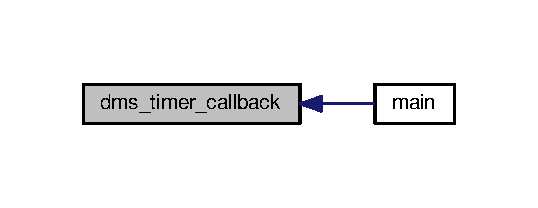
\includegraphics[width=258pt]{car__control_8cpp_ad58ce7bfd8b125e02622b612d02985b7_icgraph}
\end{center}
\end{figure}


\index{car\+\_\+control.\+cpp@{car\+\_\+control.\+cpp}!main@{main}}
\index{main@{main}!car\+\_\+control.\+cpp@{car\+\_\+control.\+cpp}}
\subsubsection[{\texorpdfstring{main(int argc, char $\ast$$\ast$argv)}{main(int argc, char **argv)}}]{\setlength{\rightskip}{0pt plus 5cm}int main (
\begin{DoxyParamCaption}
\item[{int}]{argc, }
\item[{char $\ast$$\ast$}]{argv}
\end{DoxyParamCaption}
)}\hypertarget{car__control_8cpp_a3c04138a5bfe5d72780bb7e82a18e627}{}\label{car__control_8cpp_a3c04138a5bfe5d72780bb7e82a18e627}


Definition at line 122 of file car\+\_\+control.\+cpp.



Here is the call graph for this function\+:
\nopagebreak
\begin{figure}[H]
\begin{center}
\leavevmode
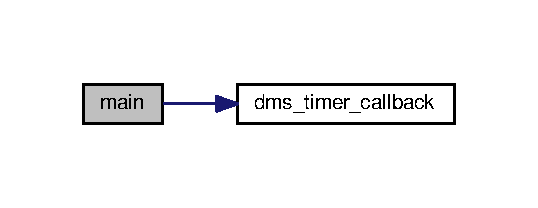
\includegraphics[width=258pt]{car__control_8cpp_a3c04138a5bfe5d72780bb7e82a18e627_cgraph}
\end{center}
\end{figure}




\subsection{Variable Documentation}
\index{car\+\_\+control.\+cpp@{car\+\_\+control.\+cpp}!dms@{dms}}
\index{dms@{dms}!car\+\_\+control.\+cpp@{car\+\_\+control.\+cpp}}
\subsubsection[{\texorpdfstring{dms}{dms}}]{\setlength{\rightskip}{0pt plus 5cm}long dms = 0}\hypertarget{car__control_8cpp_ae4b25d71b82a8bc98ea3b5bb62c409f3}{}\label{car__control_8cpp_ae4b25d71b82a8bc98ea3b5bb62c409f3}


Definition at line 53 of file car\+\_\+control.\+cpp.


\hypertarget{remote__control_8cpp}{}\section{/home/travis/build/\+Autonomous-\/\+Racing-\/\+P\+G/ros.package/docs/master/ros\+\_\+ws/src/auto\+\_\+race\+\_\+pg/src/remote\+\_\+control.cpp File Reference}
\label{remote__control_8cpp}\index{/home/travis/build/\+Autonomous-\/\+Racing-\/\+P\+G/ros.\+package/docs/master/ros\+\_\+ws/src/auto\+\_\+race\+\_\+pg/src/remote\+\_\+control.\+cpp@{/home/travis/build/\+Autonomous-\/\+Racing-\/\+P\+G/ros.\+package/docs/master/ros\+\_\+ws/src/auto\+\_\+race\+\_\+pg/src/remote\+\_\+control.\+cpp}}
{\ttfamily \#include $<$ros/ros.\+h$>$}\\*
{\ttfamily \#include $<$sensor\+\_\+msgs/\+Joy.\+h$>$}\\*
{\ttfamily \#include $<$signal.\+h$>$}\\*
{\ttfamily \#include $<$std\+\_\+msgs/\+Float64.\+h$>$}\\*
{\ttfamily \#include $<$termios.\+h$>$}\\*
Include dependency graph for remote\+\_\+control.\+cpp\+:
\nopagebreak
\begin{figure}[H]
\begin{center}
\leavevmode
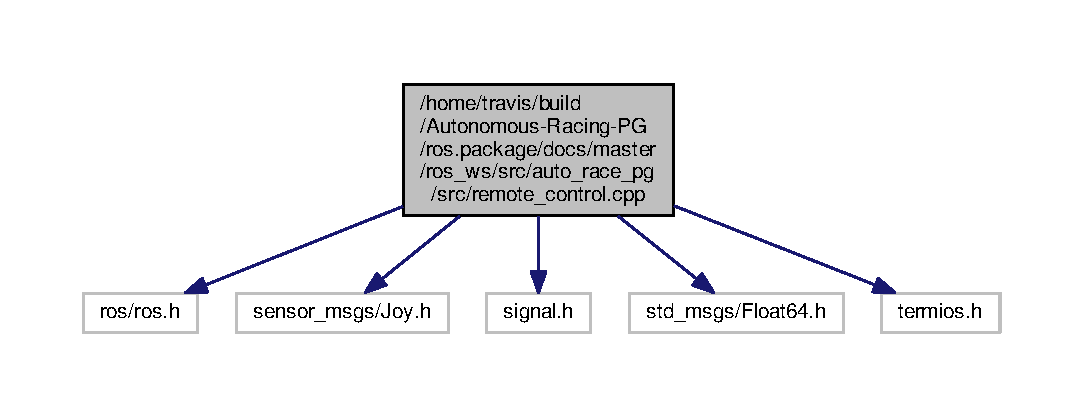
\includegraphics[width=350pt]{remote__control_8cpp__incl}
\end{center}
\end{figure}
\subsection*{Classes}
\begin{DoxyCompactItemize}
\item 
class \hyperlink{class_remote_control}{Remote\+Control}
\end{DoxyCompactItemize}
\subsection*{Macros}
\begin{DoxyCompactItemize}
\item 
\#define \hyperlink{remote__control_8cpp_ac2cd96d53dd3ba6407db6766c3d92b26}{M\+A\+X\+\_\+\+S\+P\+E\+ED}~5000
\item 
\#define \hyperlink{remote__control_8cpp_af3c82099d63a2d91d68bd62d954059c7}{M\+A\+X\+\_\+\+A\+N\+G\+LE}~0.\+8
\item 
\#define \hyperlink{remote__control_8cpp_a8c6b7fe5ad62f0dd9be385ca98ca1c9a}{T\+O\+P\+I\+C\+\_\+\+S\+P\+E\+ED}~\char`\"{}/set/speed\char`\"{}
\item 
\#define \hyperlink{remote__control_8cpp_ae85d82183138111cc259bc2920f54e9f}{T\+O\+P\+I\+C\+\_\+\+A\+N\+G\+LE}~\char`\"{}/set/position\char`\"{}
\item 
\#define \hyperlink{remote__control_8cpp_a6a44fd7e61a3f73fffecd1ec5973f819}{K\+E\+Y\+C\+O\+D\+E\+\_\+W}~119
\item 
\#define \hyperlink{remote__control_8cpp_a35ba55030dedad2411239e6330435742}{K\+E\+Y\+C\+O\+D\+E\+\_\+A}~97
\item 
\#define \hyperlink{remote__control_8cpp_a9be3d5563fec0f900d20668973b5806c}{K\+E\+Y\+C\+O\+D\+E\+\_\+S}~115
\item 
\#define \hyperlink{remote__control_8cpp_af0c998786dcada98bf809fea0b157603}{K\+E\+Y\+C\+O\+D\+E\+\_\+D}~100
\item 
\#define \hyperlink{remote__control_8cpp_a49115085a0fac000fb82c9d86c4c34d3}{K\+E\+Y\+C\+O\+D\+E\+\_\+\+S\+P\+A\+CE}~32
\end{DoxyCompactItemize}
\subsection*{Functions}
\begin{DoxyCompactItemize}
\item 
void \hyperlink{remote__control_8cpp_af9150b82e29a37ab848ee2f66e993793}{quit} (int sig)
\item 
int \hyperlink{remote__control_8cpp_a3c04138a5bfe5d72780bb7e82a18e627}{main} (int argc, char $\ast$$\ast$argv)
\end{DoxyCompactItemize}


\subsection{Macro Definition Documentation}
\index{remote\+\_\+control.\+cpp@{remote\+\_\+control.\+cpp}!K\+E\+Y\+C\+O\+D\+E\+\_\+A@{K\+E\+Y\+C\+O\+D\+E\+\_\+A}}
\index{K\+E\+Y\+C\+O\+D\+E\+\_\+A@{K\+E\+Y\+C\+O\+D\+E\+\_\+A}!remote\+\_\+control.\+cpp@{remote\+\_\+control.\+cpp}}
\subsubsection[{\texorpdfstring{K\+E\+Y\+C\+O\+D\+E\+\_\+A}{KEYCODE_A}}]{\setlength{\rightskip}{0pt plus 5cm}\#define K\+E\+Y\+C\+O\+D\+E\+\_\+A~97}\hypertarget{remote__control_8cpp_a35ba55030dedad2411239e6330435742}{}\label{remote__control_8cpp_a35ba55030dedad2411239e6330435742}


Definition at line 15 of file remote\+\_\+control.\+cpp.

\index{remote\+\_\+control.\+cpp@{remote\+\_\+control.\+cpp}!K\+E\+Y\+C\+O\+D\+E\+\_\+D@{K\+E\+Y\+C\+O\+D\+E\+\_\+D}}
\index{K\+E\+Y\+C\+O\+D\+E\+\_\+D@{K\+E\+Y\+C\+O\+D\+E\+\_\+D}!remote\+\_\+control.\+cpp@{remote\+\_\+control.\+cpp}}
\subsubsection[{\texorpdfstring{K\+E\+Y\+C\+O\+D\+E\+\_\+D}{KEYCODE_D}}]{\setlength{\rightskip}{0pt plus 5cm}\#define K\+E\+Y\+C\+O\+D\+E\+\_\+D~100}\hypertarget{remote__control_8cpp_af0c998786dcada98bf809fea0b157603}{}\label{remote__control_8cpp_af0c998786dcada98bf809fea0b157603}


Definition at line 17 of file remote\+\_\+control.\+cpp.

\index{remote\+\_\+control.\+cpp@{remote\+\_\+control.\+cpp}!K\+E\+Y\+C\+O\+D\+E\+\_\+S@{K\+E\+Y\+C\+O\+D\+E\+\_\+S}}
\index{K\+E\+Y\+C\+O\+D\+E\+\_\+S@{K\+E\+Y\+C\+O\+D\+E\+\_\+S}!remote\+\_\+control.\+cpp@{remote\+\_\+control.\+cpp}}
\subsubsection[{\texorpdfstring{K\+E\+Y\+C\+O\+D\+E\+\_\+S}{KEYCODE_S}}]{\setlength{\rightskip}{0pt plus 5cm}\#define K\+E\+Y\+C\+O\+D\+E\+\_\+S~115}\hypertarget{remote__control_8cpp_a9be3d5563fec0f900d20668973b5806c}{}\label{remote__control_8cpp_a9be3d5563fec0f900d20668973b5806c}


Definition at line 16 of file remote\+\_\+control.\+cpp.

\index{remote\+\_\+control.\+cpp@{remote\+\_\+control.\+cpp}!K\+E\+Y\+C\+O\+D\+E\+\_\+\+S\+P\+A\+CE@{K\+E\+Y\+C\+O\+D\+E\+\_\+\+S\+P\+A\+CE}}
\index{K\+E\+Y\+C\+O\+D\+E\+\_\+\+S\+P\+A\+CE@{K\+E\+Y\+C\+O\+D\+E\+\_\+\+S\+P\+A\+CE}!remote\+\_\+control.\+cpp@{remote\+\_\+control.\+cpp}}
\subsubsection[{\texorpdfstring{K\+E\+Y\+C\+O\+D\+E\+\_\+\+S\+P\+A\+CE}{KEYCODE_SPACE}}]{\setlength{\rightskip}{0pt plus 5cm}\#define K\+E\+Y\+C\+O\+D\+E\+\_\+\+S\+P\+A\+CE~32}\hypertarget{remote__control_8cpp_a49115085a0fac000fb82c9d86c4c34d3}{}\label{remote__control_8cpp_a49115085a0fac000fb82c9d86c4c34d3}


Definition at line 18 of file remote\+\_\+control.\+cpp.

\index{remote\+\_\+control.\+cpp@{remote\+\_\+control.\+cpp}!K\+E\+Y\+C\+O\+D\+E\+\_\+W@{K\+E\+Y\+C\+O\+D\+E\+\_\+W}}
\index{K\+E\+Y\+C\+O\+D\+E\+\_\+W@{K\+E\+Y\+C\+O\+D\+E\+\_\+W}!remote\+\_\+control.\+cpp@{remote\+\_\+control.\+cpp}}
\subsubsection[{\texorpdfstring{K\+E\+Y\+C\+O\+D\+E\+\_\+W}{KEYCODE_W}}]{\setlength{\rightskip}{0pt plus 5cm}\#define K\+E\+Y\+C\+O\+D\+E\+\_\+W~119}\hypertarget{remote__control_8cpp_a6a44fd7e61a3f73fffecd1ec5973f819}{}\label{remote__control_8cpp_a6a44fd7e61a3f73fffecd1ec5973f819}


Definition at line 14 of file remote\+\_\+control.\+cpp.

\index{remote\+\_\+control.\+cpp@{remote\+\_\+control.\+cpp}!M\+A\+X\+\_\+\+A\+N\+G\+LE@{M\+A\+X\+\_\+\+A\+N\+G\+LE}}
\index{M\+A\+X\+\_\+\+A\+N\+G\+LE@{M\+A\+X\+\_\+\+A\+N\+G\+LE}!remote\+\_\+control.\+cpp@{remote\+\_\+control.\+cpp}}
\subsubsection[{\texorpdfstring{M\+A\+X\+\_\+\+A\+N\+G\+LE}{MAX_ANGLE}}]{\setlength{\rightskip}{0pt plus 5cm}\#define M\+A\+X\+\_\+\+A\+N\+G\+LE~0.\+8}\hypertarget{remote__control_8cpp_af3c82099d63a2d91d68bd62d954059c7}{}\label{remote__control_8cpp_af3c82099d63a2d91d68bd62d954059c7}


Definition at line 9 of file remote\+\_\+control.\+cpp.

\index{remote\+\_\+control.\+cpp@{remote\+\_\+control.\+cpp}!M\+A\+X\+\_\+\+S\+P\+E\+ED@{M\+A\+X\+\_\+\+S\+P\+E\+ED}}
\index{M\+A\+X\+\_\+\+S\+P\+E\+ED@{M\+A\+X\+\_\+\+S\+P\+E\+ED}!remote\+\_\+control.\+cpp@{remote\+\_\+control.\+cpp}}
\subsubsection[{\texorpdfstring{M\+A\+X\+\_\+\+S\+P\+E\+ED}{MAX_SPEED}}]{\setlength{\rightskip}{0pt plus 5cm}\#define M\+A\+X\+\_\+\+S\+P\+E\+ED~5000}\hypertarget{remote__control_8cpp_ac2cd96d53dd3ba6407db6766c3d92b26}{}\label{remote__control_8cpp_ac2cd96d53dd3ba6407db6766c3d92b26}


Definition at line 8 of file remote\+\_\+control.\+cpp.

\index{remote\+\_\+control.\+cpp@{remote\+\_\+control.\+cpp}!T\+O\+P\+I\+C\+\_\+\+A\+N\+G\+LE@{T\+O\+P\+I\+C\+\_\+\+A\+N\+G\+LE}}
\index{T\+O\+P\+I\+C\+\_\+\+A\+N\+G\+LE@{T\+O\+P\+I\+C\+\_\+\+A\+N\+G\+LE}!remote\+\_\+control.\+cpp@{remote\+\_\+control.\+cpp}}
\subsubsection[{\texorpdfstring{T\+O\+P\+I\+C\+\_\+\+A\+N\+G\+LE}{TOPIC_ANGLE}}]{\setlength{\rightskip}{0pt plus 5cm}\#define T\+O\+P\+I\+C\+\_\+\+A\+N\+G\+LE~\char`\"{}/set/position\char`\"{}}\hypertarget{remote__control_8cpp_ae85d82183138111cc259bc2920f54e9f}{}\label{remote__control_8cpp_ae85d82183138111cc259bc2920f54e9f}


Definition at line 12 of file remote\+\_\+control.\+cpp.

\index{remote\+\_\+control.\+cpp@{remote\+\_\+control.\+cpp}!T\+O\+P\+I\+C\+\_\+\+S\+P\+E\+ED@{T\+O\+P\+I\+C\+\_\+\+S\+P\+E\+ED}}
\index{T\+O\+P\+I\+C\+\_\+\+S\+P\+E\+ED@{T\+O\+P\+I\+C\+\_\+\+S\+P\+E\+ED}!remote\+\_\+control.\+cpp@{remote\+\_\+control.\+cpp}}
\subsubsection[{\texorpdfstring{T\+O\+P\+I\+C\+\_\+\+S\+P\+E\+ED}{TOPIC_SPEED}}]{\setlength{\rightskip}{0pt plus 5cm}\#define T\+O\+P\+I\+C\+\_\+\+S\+P\+E\+ED~\char`\"{}/set/speed\char`\"{}}\hypertarget{remote__control_8cpp_a8c6b7fe5ad62f0dd9be385ca98ca1c9a}{}\label{remote__control_8cpp_a8c6b7fe5ad62f0dd9be385ca98ca1c9a}


Definition at line 11 of file remote\+\_\+control.\+cpp.



\subsection{Function Documentation}
\index{remote\+\_\+control.\+cpp@{remote\+\_\+control.\+cpp}!main@{main}}
\index{main@{main}!remote\+\_\+control.\+cpp@{remote\+\_\+control.\+cpp}}
\subsubsection[{\texorpdfstring{main(int argc, char $\ast$$\ast$argv)}{main(int argc, char **argv)}}]{\setlength{\rightskip}{0pt plus 5cm}int main (
\begin{DoxyParamCaption}
\item[{int}]{argc, }
\item[{char $\ast$$\ast$}]{argv}
\end{DoxyParamCaption}
)}\hypertarget{remote__control_8cpp_a3c04138a5bfe5d72780bb7e82a18e627}{}\label{remote__control_8cpp_a3c04138a5bfe5d72780bb7e82a18e627}


Definition at line 144 of file remote\+\_\+control.\+cpp.



Here is the call graph for this function\+:
\nopagebreak
\begin{figure}[H]
\begin{center}
\leavevmode
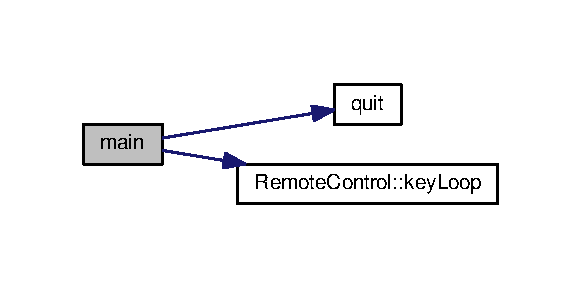
\includegraphics[width=279pt]{remote__control_8cpp_a3c04138a5bfe5d72780bb7e82a18e627_cgraph}
\end{center}
\end{figure}


\index{remote\+\_\+control.\+cpp@{remote\+\_\+control.\+cpp}!quit@{quit}}
\index{quit@{quit}!remote\+\_\+control.\+cpp@{remote\+\_\+control.\+cpp}}
\subsubsection[{\texorpdfstring{quit(int sig)}{quit(int sig)}}]{\setlength{\rightskip}{0pt plus 5cm}void quit (
\begin{DoxyParamCaption}
\item[{int}]{sig}
\end{DoxyParamCaption}
)}\hypertarget{remote__control_8cpp_af9150b82e29a37ab848ee2f66e993793}{}\label{remote__control_8cpp_af9150b82e29a37ab848ee2f66e993793}


Definition at line 138 of file remote\+\_\+control.\+cpp.



Here is the caller graph for this function\+:
\nopagebreak
\begin{figure}[H]
\begin{center}
\leavevmode
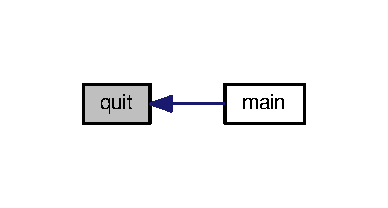
\includegraphics[width=186pt]{remote__control_8cpp_af9150b82e29a37ab848ee2f66e993793_icgraph}
\end{center}
\end{figure}



\hypertarget{remote__joy_8cpp}{}\section{/home/travis/build/\+Autonomous-\/\+Racing-\/\+P\+G/ros.package/ros\+\_\+ws/src/auto\+\_\+race\+\_\+pg/src/remote\+\_\+joy.cpp File Reference}
\label{remote__joy_8cpp}\index{/home/travis/build/\+Autonomous-\/\+Racing-\/\+P\+G/ros.\+package/ros\+\_\+ws/src/auto\+\_\+race\+\_\+pg/src/remote\+\_\+joy.\+cpp@{/home/travis/build/\+Autonomous-\/\+Racing-\/\+P\+G/ros.\+package/ros\+\_\+ws/src/auto\+\_\+race\+\_\+pg/src/remote\+\_\+joy.\+cpp}}
{\ttfamily \#include $<$ros/ros.\+h$>$}\\*
{\ttfamily \#include $<$sensor\+\_\+msgs/\+Joy.\+h$>$}\\*
{\ttfamily \#include $<$std\+\_\+msgs/\+Float64.\+h$>$}\\*
Include dependency graph for remote\+\_\+joy.\+cpp\+:
\nopagebreak
\begin{figure}[H]
\begin{center}
\leavevmode
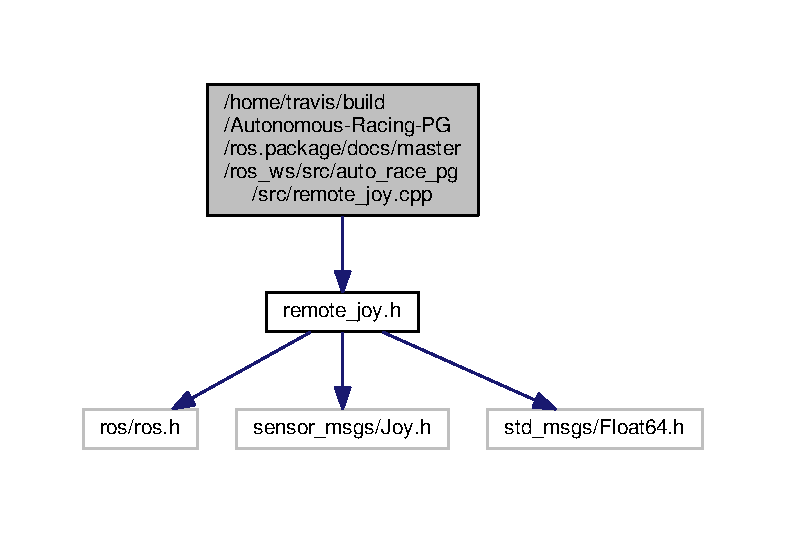
\includegraphics[width=350pt]{remote__joy_8cpp__incl}
\end{center}
\end{figure}
\subsection*{Classes}
\begin{DoxyCompactItemize}
\item 
class \hyperlink{class_remote_joy}{Remote\+Joy}
\end{DoxyCompactItemize}
\subsection*{Macros}
\begin{DoxyCompactItemize}
\item 
\#define \hyperlink{remote__joy_8cpp_ab8c52c1b4c021ed3e6b6b677bd2ac019}{M\+O\+DE}~\char`\"{}joy\char`\"{}
\item 
\#define \hyperlink{remote__joy_8cpp_acbfb5eae88329444b807a7b3a180d855}{J\+O\+Y\+\_\+\+A\+N\+G\+L\+E\+\_\+\+A\+N\+G\+U\+L\+AR}~0
\item 
\#define \hyperlink{remote__joy_8cpp_a447fc4cb069a0478754727f0383f7e1b}{J\+O\+Y\+\_\+\+A\+N\+G\+L\+E\+\_\+\+L\+I\+N\+E\+AR}~1
\item 
\#define \hyperlink{remote__joy_8cpp_a8c6b7fe5ad62f0dd9be385ca98ca1c9a}{T\+O\+P\+I\+C\+\_\+\+S\+P\+E\+ED}~\char`\"{}/set/speed\char`\"{}
\item 
\#define \hyperlink{remote__joy_8cpp_ae85d82183138111cc259bc2920f54e9f}{T\+O\+P\+I\+C\+\_\+\+A\+N\+G\+LE}~\char`\"{}/set/angle\char`\"{}
\end{DoxyCompactItemize}
\subsection*{Functions}
\begin{DoxyCompactItemize}
\item 
int \hyperlink{remote__joy_8cpp_a3c04138a5bfe5d72780bb7e82a18e627}{main} (int argc, char $\ast$$\ast$argv)
\end{DoxyCompactItemize}


\subsection{Macro Definition Documentation}
\index{remote\+\_\+joy.\+cpp@{remote\+\_\+joy.\+cpp}!J\+O\+Y\+\_\+\+A\+N\+G\+L\+E\+\_\+\+A\+N\+G\+U\+L\+AR@{J\+O\+Y\+\_\+\+A\+N\+G\+L\+E\+\_\+\+A\+N\+G\+U\+L\+AR}}
\index{J\+O\+Y\+\_\+\+A\+N\+G\+L\+E\+\_\+\+A\+N\+G\+U\+L\+AR@{J\+O\+Y\+\_\+\+A\+N\+G\+L\+E\+\_\+\+A\+N\+G\+U\+L\+AR}!remote\+\_\+joy.\+cpp@{remote\+\_\+joy.\+cpp}}
\subsubsection[{\texorpdfstring{J\+O\+Y\+\_\+\+A\+N\+G\+L\+E\+\_\+\+A\+N\+G\+U\+L\+AR}{JOY_ANGLE_ANGULAR}}]{\setlength{\rightskip}{0pt plus 5cm}\#define J\+O\+Y\+\_\+\+A\+N\+G\+L\+E\+\_\+\+A\+N\+G\+U\+L\+AR~0}\hypertarget{remote__joy_8cpp_acbfb5eae88329444b807a7b3a180d855}{}\label{remote__joy_8cpp_acbfb5eae88329444b807a7b3a180d855}


Definition at line 8 of file remote\+\_\+joy.\+cpp.

\index{remote\+\_\+joy.\+cpp@{remote\+\_\+joy.\+cpp}!J\+O\+Y\+\_\+\+A\+N\+G\+L\+E\+\_\+\+L\+I\+N\+E\+AR@{J\+O\+Y\+\_\+\+A\+N\+G\+L\+E\+\_\+\+L\+I\+N\+E\+AR}}
\index{J\+O\+Y\+\_\+\+A\+N\+G\+L\+E\+\_\+\+L\+I\+N\+E\+AR@{J\+O\+Y\+\_\+\+A\+N\+G\+L\+E\+\_\+\+L\+I\+N\+E\+AR}!remote\+\_\+joy.\+cpp@{remote\+\_\+joy.\+cpp}}
\subsubsection[{\texorpdfstring{J\+O\+Y\+\_\+\+A\+N\+G\+L\+E\+\_\+\+L\+I\+N\+E\+AR}{JOY_ANGLE_LINEAR}}]{\setlength{\rightskip}{0pt plus 5cm}\#define J\+O\+Y\+\_\+\+A\+N\+G\+L\+E\+\_\+\+L\+I\+N\+E\+AR~1}\hypertarget{remote__joy_8cpp_a447fc4cb069a0478754727f0383f7e1b}{}\label{remote__joy_8cpp_a447fc4cb069a0478754727f0383f7e1b}


Definition at line 9 of file remote\+\_\+joy.\+cpp.

\index{remote\+\_\+joy.\+cpp@{remote\+\_\+joy.\+cpp}!M\+O\+DE@{M\+O\+DE}}
\index{M\+O\+DE@{M\+O\+DE}!remote\+\_\+joy.\+cpp@{remote\+\_\+joy.\+cpp}}
\subsubsection[{\texorpdfstring{M\+O\+DE}{MODE}}]{\setlength{\rightskip}{0pt plus 5cm}\#define M\+O\+DE~\char`\"{}joy\char`\"{}}\hypertarget{remote__joy_8cpp_ab8c52c1b4c021ed3e6b6b677bd2ac019}{}\label{remote__joy_8cpp_ab8c52c1b4c021ed3e6b6b677bd2ac019}


Definition at line 6 of file remote\+\_\+joy.\+cpp.

\index{remote\+\_\+joy.\+cpp@{remote\+\_\+joy.\+cpp}!T\+O\+P\+I\+C\+\_\+\+A\+N\+G\+LE@{T\+O\+P\+I\+C\+\_\+\+A\+N\+G\+LE}}
\index{T\+O\+P\+I\+C\+\_\+\+A\+N\+G\+LE@{T\+O\+P\+I\+C\+\_\+\+A\+N\+G\+LE}!remote\+\_\+joy.\+cpp@{remote\+\_\+joy.\+cpp}}
\subsubsection[{\texorpdfstring{T\+O\+P\+I\+C\+\_\+\+A\+N\+G\+LE}{TOPIC_ANGLE}}]{\setlength{\rightskip}{0pt plus 5cm}\#define T\+O\+P\+I\+C\+\_\+\+A\+N\+G\+LE~\char`\"{}/set/angle\char`\"{}}\hypertarget{remote__joy_8cpp_ae85d82183138111cc259bc2920f54e9f}{}\label{remote__joy_8cpp_ae85d82183138111cc259bc2920f54e9f}


Definition at line 12 of file remote\+\_\+joy.\+cpp.

\index{remote\+\_\+joy.\+cpp@{remote\+\_\+joy.\+cpp}!T\+O\+P\+I\+C\+\_\+\+S\+P\+E\+ED@{T\+O\+P\+I\+C\+\_\+\+S\+P\+E\+ED}}
\index{T\+O\+P\+I\+C\+\_\+\+S\+P\+E\+ED@{T\+O\+P\+I\+C\+\_\+\+S\+P\+E\+ED}!remote\+\_\+joy.\+cpp@{remote\+\_\+joy.\+cpp}}
\subsubsection[{\texorpdfstring{T\+O\+P\+I\+C\+\_\+\+S\+P\+E\+ED}{TOPIC_SPEED}}]{\setlength{\rightskip}{0pt plus 5cm}\#define T\+O\+P\+I\+C\+\_\+\+S\+P\+E\+ED~\char`\"{}/set/speed\char`\"{}}\hypertarget{remote__joy_8cpp_a8c6b7fe5ad62f0dd9be385ca98ca1c9a}{}\label{remote__joy_8cpp_a8c6b7fe5ad62f0dd9be385ca98ca1c9a}


Definition at line 11 of file remote\+\_\+joy.\+cpp.



\subsection{Function Documentation}
\index{remote\+\_\+joy.\+cpp@{remote\+\_\+joy.\+cpp}!main@{main}}
\index{main@{main}!remote\+\_\+joy.\+cpp@{remote\+\_\+joy.\+cpp}}
\subsubsection[{\texorpdfstring{main(int argc, char $\ast$$\ast$argv)}{main(int argc, char **argv)}}]{\setlength{\rightskip}{0pt plus 5cm}int main (
\begin{DoxyParamCaption}
\item[{int}]{argc, }
\item[{char $\ast$$\ast$}]{argv}
\end{DoxyParamCaption}
)}\hypertarget{remote__joy_8cpp_a3c04138a5bfe5d72780bb7e82a18e627}{}\label{remote__joy_8cpp_a3c04138a5bfe5d72780bb7e82a18e627}


Definition at line 67 of file remote\+\_\+joy.\+cpp.


\hypertarget{remote__keyboard_8cpp}{}\section{/home/travis/build/\+Autonomous-\/\+Racing-\/\+P\+G/ros.package/docs/master/ros\+\_\+ws/src/auto\+\_\+race\+\_\+pg/src/remote\+\_\+keyboard.cpp File Reference}
\label{remote__keyboard_8cpp}\index{/home/travis/build/\+Autonomous-\/\+Racing-\/\+P\+G/ros.\+package/docs/master/ros\+\_\+ws/src/auto\+\_\+race\+\_\+pg/src/remote\+\_\+keyboard.\+cpp@{/home/travis/build/\+Autonomous-\/\+Racing-\/\+P\+G/ros.\+package/docs/master/ros\+\_\+ws/src/auto\+\_\+race\+\_\+pg/src/remote\+\_\+keyboard.\+cpp}}
{\ttfamily \#include \char`\"{}remote\+\_\+keyboard.\+h\char`\"{}}\\*
Include dependency graph for remote\+\_\+keyboard.\+cpp\+:
\nopagebreak
\begin{figure}[H]
\begin{center}
\leavevmode
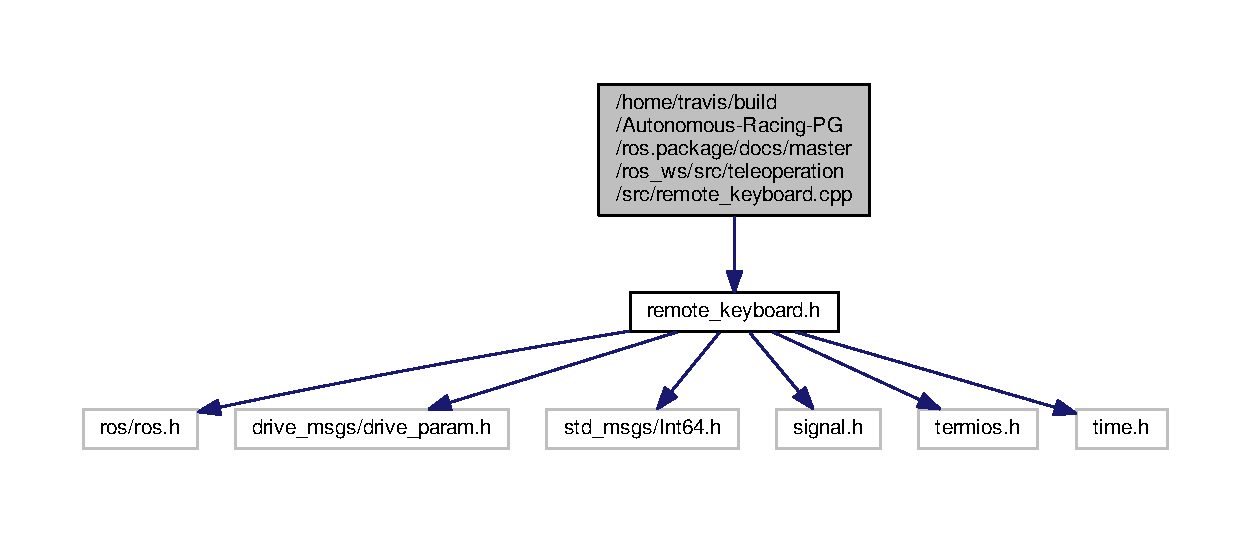
\includegraphics[width=350pt]{remote__keyboard_8cpp__incl}
\end{center}
\end{figure}
\subsection*{Functions}
\begin{DoxyCompactItemize}
\item 
void \hyperlink{remote__keyboard_8cpp_af9150b82e29a37ab848ee2f66e993793}{quit} (int sig)
\item 
int \hyperlink{remote__keyboard_8cpp_a3c04138a5bfe5d72780bb7e82a18e627}{main} (int argc, char $\ast$$\ast$argv)
\end{DoxyCompactItemize}


\subsection{Function Documentation}
\index{remote\+\_\+keyboard.\+cpp@{remote\+\_\+keyboard.\+cpp}!main@{main}}
\index{main@{main}!remote\+\_\+keyboard.\+cpp@{remote\+\_\+keyboard.\+cpp}}
\subsubsection[{\texorpdfstring{main(int argc, char $\ast$$\ast$argv)}{main(int argc, char **argv)}}]{\setlength{\rightskip}{0pt plus 5cm}int main (
\begin{DoxyParamCaption}
\item[{int}]{argc, }
\item[{char $\ast$$\ast$}]{argv}
\end{DoxyParamCaption}
)}\hypertarget{remote__keyboard_8cpp_a3c04138a5bfe5d72780bb7e82a18e627}{}\label{remote__keyboard_8cpp_a3c04138a5bfe5d72780bb7e82a18e627}


Definition at line 87 of file remote\+\_\+keyboard.\+cpp.



Here is the call graph for this function\+:
\nopagebreak
\begin{figure}[H]
\begin{center}
\leavevmode
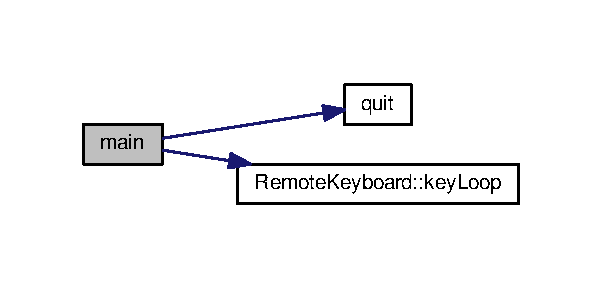
\includegraphics[width=289pt]{remote__keyboard_8cpp_a3c04138a5bfe5d72780bb7e82a18e627_cgraph}
\end{center}
\end{figure}


\index{remote\+\_\+keyboard.\+cpp@{remote\+\_\+keyboard.\+cpp}!quit@{quit}}
\index{quit@{quit}!remote\+\_\+keyboard.\+cpp@{remote\+\_\+keyboard.\+cpp}}
\subsubsection[{\texorpdfstring{quit(int sig)}{quit(int sig)}}]{\setlength{\rightskip}{0pt plus 5cm}void quit (
\begin{DoxyParamCaption}
\item[{int}]{sig}
\end{DoxyParamCaption}
)}\hypertarget{remote__keyboard_8cpp_af9150b82e29a37ab848ee2f66e993793}{}\label{remote__keyboard_8cpp_af9150b82e29a37ab848ee2f66e993793}


Definition at line 81 of file remote\+\_\+keyboard.\+cpp.



Here is the caller graph for this function\+:
\nopagebreak
\begin{figure}[H]
\begin{center}
\leavevmode
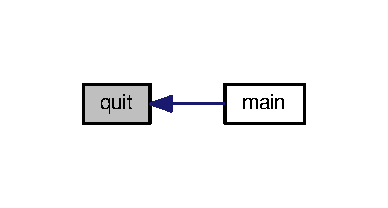
\includegraphics[width=186pt]{remote__keyboard_8cpp_af9150b82e29a37ab848ee2f66e993793_icgraph}
\end{center}
\end{figure}



\hypertarget{test__auto__race__pg_8cpp}{}\section{/home/travis/build/\+Autonomous-\/\+Racing-\/\+P\+G/ros.package/ros\+\_\+ws/src/auto\+\_\+race\+\_\+pg/test/test\+\_\+auto\+\_\+race\+\_\+pg.cpp File Reference}
\label{test__auto__race__pg_8cpp}\index{/home/travis/build/\+Autonomous-\/\+Racing-\/\+P\+G/ros.\+package/ros\+\_\+ws/src/auto\+\_\+race\+\_\+pg/test/test\+\_\+auto\+\_\+race\+\_\+pg.\+cpp@{/home/travis/build/\+Autonomous-\/\+Racing-\/\+P\+G/ros.\+package/ros\+\_\+ws/src/auto\+\_\+race\+\_\+pg/test/test\+\_\+auto\+\_\+race\+\_\+pg.\+cpp}}
{\ttfamily \#include $<$cstdlib$>$}\\*
{\ttfamily \#include $<$gtest/gtest.\+h$>$}\\*
Include dependency graph for test\+\_\+auto\+\_\+race\+\_\+pg.\+cpp\+:
\nopagebreak
\begin{figure}[H]
\begin{center}
\leavevmode
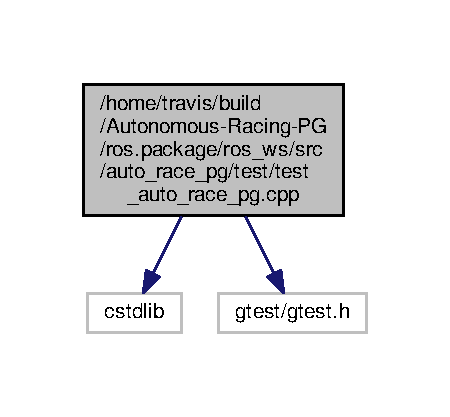
\includegraphics[width=216pt]{test__auto__race__pg_8cpp__incl}
\end{center}
\end{figure}
\subsection*{Functions}
\begin{DoxyCompactItemize}
\item 
\hyperlink{test__auto__race__pg_8cpp_abdd1a026bf2a8a181d4f4f61169c22f9}{T\+E\+ST} (dummy\+\_\+test, dummy\+\_\+test\+\_\+01)
\item 
\hyperlink{test__auto__race__pg_8cpp_a6accdba7cce21b4fbadc9847942eccee}{T\+E\+ST} (dummy\+\_\+test, dummy\+\_\+test\+\_\+02)
\item 
int \hyperlink{test__auto__race__pg_8cpp_a3c04138a5bfe5d72780bb7e82a18e627}{main} (int argc, char $\ast$$\ast$argv)
\end{DoxyCompactItemize}


\subsection{Function Documentation}
\index{test\+\_\+auto\+\_\+race\+\_\+pg.\+cpp@{test\+\_\+auto\+\_\+race\+\_\+pg.\+cpp}!main@{main}}
\index{main@{main}!test\+\_\+auto\+\_\+race\+\_\+pg.\+cpp@{test\+\_\+auto\+\_\+race\+\_\+pg.\+cpp}}
\subsubsection[{\texorpdfstring{main(int argc, char $\ast$$\ast$argv)}{main(int argc, char **argv)}}]{\setlength{\rightskip}{0pt plus 5cm}int main (
\begin{DoxyParamCaption}
\item[{int}]{argc, }
\item[{char $\ast$$\ast$}]{argv}
\end{DoxyParamCaption}
)}\hypertarget{test__auto__race__pg_8cpp_a3c04138a5bfe5d72780bb7e82a18e627}{}\label{test__auto__race__pg_8cpp_a3c04138a5bfe5d72780bb7e82a18e627}


Definition at line 20 of file test\+\_\+auto\+\_\+race\+\_\+pg.\+cpp.

\index{test\+\_\+auto\+\_\+race\+\_\+pg.\+cpp@{test\+\_\+auto\+\_\+race\+\_\+pg.\+cpp}!T\+E\+ST@{T\+E\+ST}}
\index{T\+E\+ST@{T\+E\+ST}!test\+\_\+auto\+\_\+race\+\_\+pg.\+cpp@{test\+\_\+auto\+\_\+race\+\_\+pg.\+cpp}}
\subsubsection[{\texorpdfstring{T\+E\+S\+T(dummy\+\_\+test, dummy\+\_\+test\+\_\+01)}{TEST(dummy_test, dummy_test_01)}}]{\setlength{\rightskip}{0pt plus 5cm}T\+E\+ST (
\begin{DoxyParamCaption}
\item[{dummy\+\_\+test}]{, }
\item[{dummy\+\_\+test\+\_\+01}]{}
\end{DoxyParamCaption}
)}\hypertarget{test__auto__race__pg_8cpp_abdd1a026bf2a8a181d4f4f61169c22f9}{}\label{test__auto__race__pg_8cpp_abdd1a026bf2a8a181d4f4f61169c22f9}


Definition at line 10 of file test\+\_\+auto\+\_\+race\+\_\+pg.\+cpp.

\index{test\+\_\+auto\+\_\+race\+\_\+pg.\+cpp@{test\+\_\+auto\+\_\+race\+\_\+pg.\+cpp}!T\+E\+ST@{T\+E\+ST}}
\index{T\+E\+ST@{T\+E\+ST}!test\+\_\+auto\+\_\+race\+\_\+pg.\+cpp@{test\+\_\+auto\+\_\+race\+\_\+pg.\+cpp}}
\subsubsection[{\texorpdfstring{T\+E\+S\+T(dummy\+\_\+test, dummy\+\_\+test\+\_\+02)}{TEST(dummy_test, dummy_test_02)}}]{\setlength{\rightskip}{0pt plus 5cm}T\+E\+ST (
\begin{DoxyParamCaption}
\item[{dummy\+\_\+test}]{, }
\item[{dummy\+\_\+test\+\_\+02}]{}
\end{DoxyParamCaption}
)}\hypertarget{test__auto__race__pg_8cpp_a6accdba7cce21b4fbadc9847942eccee}{}\label{test__auto__race__pg_8cpp_a6accdba7cce21b4fbadc9847942eccee}


Definition at line 15 of file test\+\_\+auto\+\_\+race\+\_\+pg.\+cpp.


\hypertarget{drive__param__converter_8py}{}\section{/home/travis/build/\+Autonomous-\/\+Racing-\/\+P\+G/ros.package/docs/master/ros\+\_\+ws/src/simulation/racer\+\_\+control/scripts/drive\+\_\+param\+\_\+converter.py File Reference}
\label{drive__param__converter_8py}\index{/home/travis/build/\+Autonomous-\/\+Racing-\/\+P\+G/ros.\+package/docs/master/ros\+\_\+ws/src/simulation/racer\+\_\+control/scripts/drive\+\_\+param\+\_\+converter.\+py@{/home/travis/build/\+Autonomous-\/\+Racing-\/\+P\+G/ros.\+package/docs/master/ros\+\_\+ws/src/simulation/racer\+\_\+control/scripts/drive\+\_\+param\+\_\+converter.\+py}}
\subsection*{Namespaces}
\begin{DoxyCompactItemize}
\item 
 \hyperlink{namespacedrive__param__converter}{drive\+\_\+param\+\_\+converter}
\end{DoxyCompactItemize}
\subsection*{Functions}
\begin{DoxyCompactItemize}
\item 
def \hyperlink{namespacedrive__param__converter_afdd5fa91c648e8545fae1cd833995f40}{drive\+\_\+param\+\_\+converter.\+set\+\_\+throttle\+\_\+steer} (data)
\item 
def \hyperlink{namespacedrive__param__converter_a14d9041f6f5fd041bfbea4f26cbe0155}{drive\+\_\+param\+\_\+converter.\+drive\+\_\+param\+\_\+converter} ()
\end{DoxyCompactItemize}
\subsection*{Variables}
\begin{DoxyCompactItemize}
\item 
int \hyperlink{namespacedrive__param__converter_aab4bf01f556d80bbeeb22edf8bf07611}{drive\+\_\+param\+\_\+converter.\+flag\+\_\+move} = 0
\end{DoxyCompactItemize}

%--- End generated contents ---

% Index
\backmatter
\newpage
\phantomsection
\clearemptydoublepage
\addcontentsline{toc}{chapter}{Index}
\printindex

\end{document}
